% R44: original printed pp. 489--500, §4 continued through Theorem 4

\section{外微分形式}

\noindent\textbf{1. 从一个张量空间到张量丛}\quad
设 $M$ 是一个 $n$ 维 $C^\infty$ 微分流形，于是对其上每一点 $P\in M$，有切空间 $T_P(M)$ 与余切空间 $T_P^*(M)$ 是其对偶。如果孤立地看一个点，即固定 $P$，则切空间与余切空间就是 $\mathbb R^n$ 与 $(\mathbb R^n)^*$，其上的向量与张量结构我们已在 §1 与 §3 中作了详尽的讨论。若令 $P$ 在 $M$ 中变动，我们就会得到一族线性空间
\[
 \bigcup_P T_P(M)\qquad\hbox{与}\qquad \bigcup_P T_P^*(M).
\]
因为 $M$ 是光滑的，我们直觉地会想到，例如 $T_P(M)$ 中某一切向量当 $P$ 变动时也会光滑地变化。但是实际上并不如此简单。不同的 $P$ 点的切空间之基底互相没有关系，当 $P$ 一旦变动，原来 $T_P(M)$ 的基底（例如记作 $\{e_{1P},\ldots,e_{nP}\}$）不知道会怎样变，甚至原来线性无关的向量也会变成线性相关而使 $\{e_{1P},\ldots,e_{nP}\}$ 不再成为基底。所以在 §2 中讨论向量丛时，我们不能只考虑底空间 $M$ 上之点 $P$ 附近 $U_\alpha$ 中的局部坐标映射，还要考虑纤维之变化，于是要求 $\pi^{-1}(U_\alpha)$ 能同胚于 $U_\alpha\times\mathbb R^n$，且 $\pi^{-1}(P)\cong\mathbb R^n$。这样一来，当 $P$ 在 $U_\alpha$ 中变化时，可以使 $P$ 点在每个位置上的基底之间有线性同构关系，且此同构之系数是 $C^\infty(M)$ 函数。这样一来，底空间的局部坐标 $x$ 与纤维之坐标 $\xi$ 就完全分开，而在 $\bigcup_{x\in U_\alpha}T_x(M)$ 中可以引入如下的局部坐标系 $(x^1,\ldots,x^n;\xi_1,\ldots,\xi_n)$。这一点正是向量丛定义中的要点，即所谓局部平凡化条件。有了这一点，我们上面提出的困难就自然消解了，但又会产生一个新问题：原来固定 $P$ 点讨论 $T_P(M)$ 时是把它作为一个线性空间，其系数均为实数，现在“系数”要随 $P$ 变动了，自然就应取为 $C^\infty(U_\alpha)$ 函数。看起来这只是毫不起眼的小事，实际上带来很大的问题：线性空间的系数构成一个域（field），在代数学中域是有特定含义的，简单地说就是在域中可以作四则运算，唯有以零作为母除外。现在 $C^\infty(U_\alpha)$ 只是一个环（ring），而一个环简单说来就是可以在其中作加、减、乘的集合，而除法一般是不许可的。设若有一个不恒为 $0$ 的 $C^\infty$ 函数 $f(x)$，$f(x)$ 当然不是零元，但它可能在某一点 $P$ 为 $0$：$f(P)=0$，于是对这个非 $0$ 元也不能作 $1/f(x)$，即 $1/f(x)\notin C^\infty$。这是一个不小的限制。例如元素为实数（这是我们一直在用的域）的矩阵 $A$，是可以讨论其逆矩阵的（尽管当 $\det A=0$ 时逆矩阵并不存在），但元素在某一环（例如 $C^\infty(U_\alpha)$）中的矩阵，就根本不能谈它的逆矩阵问题，因为逆矩阵的元是以 $\det A$ 为分母的。读者一定要记住，元素在环中的矩阵和元素在域中的矩阵全然不同，例如，对于前者就不会有很有用的若尔当标准形。§2 中已说过，这种系数为 $C^\infty$ 函数的“线性空间”称为一个模（module）。模和线性空间大不相同，在讨论向量丛时应该注意这一点。但是我们又不打算去讨论模的问题，所以对读者们说来，最简单的办法是不要轻易地做除法，而要特别注意分母是否在某点可能为 $0$！以上我们重述了关于丛的问题。

现在即以 $T_P(M)$ 为基本的线性空间，即上节中的 $\mathbb R^n$，或 $V$，而在每一点 $P\in M$ 可以作一个张量代数 $\mathcal T_P$，一个格拉斯曼代数 $\Lambda_P(M)$。于是我们有张量代数丛 $\mathcal T(M)$ 和格拉斯曼代数丛（或外代数丛）$\Lambda(M)$。在 §2 中我们定义了一个向量丛的切口的概念。设有 $M$ 上的向量丛 $E$，其相应的投影是 $\pi$，若有由 $U\subset M$ 到 $E$ 中的映射 $\sigma$，适合 $\pi\circ\sigma=\operatorname{id}$ 就说 $\sigma$ 是 $E$ 在 $U$ 上的切口，若 $\sigma$ 是光滑的，就说此切口是光滑的。如果用比较直观的语言，现以切丛为例，并设 $U$ 是一个坐标邻域，其局部坐标为 $x=(x^1,\ldots,x^n)$，所谓给它一个切口，就是对 $U$ 中每一点（记为 $x$），可以在 $E$ 中 $x$ 处的纤维中找到一个元与之对应。因为在 $U$ 中各点处的纤维都同构于 $\mathbb R^n$，而且有一个与 $x$ 无关的，即适用于整个 $U$ 上的基底 $\{e_i\}$，所以纤维中的元若用 $\{e_i\}$ 表示必为一个特定的
\[
 (\xi_1(x),\ldots,\xi_n(x))\cong\sum_{i=1}^n\xi_i(x)e_i.
\]
所谓光滑切口则是指所有这些 $\xi_i(x)\in C^\infty(U)$。这样我们得到坐标邻域 $U$ 中的切口，就是一个局部切口。是否有可能由局部切口转而构造出 $M$ 上的整体切口？我们当然会想到找到两个相交的坐标邻域 $U$ 与 $V$ 以及其中的局部坐标 $\{x\}$ 与 $\{y\}$，于是，在 $U\cap V$ 中上述特定的纤维中的元 $(\xi_1(x),\ldots,\xi_n(x))$ 或写为 $(\eta_1(y),\ldots,\eta_n(y))$ 之间可以用迁移函数的雅可比矩阵来转换。但是这样做是否可以在整个 $M$ 上作出一个切口是一个严重的问题，不但这种整体问题有如此的困难，有时甚至局部问题也有困难。我们趁这个机会向读者介绍一件值得注意的事，能不能找到适用于坐标邻域 $U$ 中的 o.n. 系？o.n. 系显然来自内积，而内积则决定了一个度量，在一个局部坐标系下，由每一点处的一个二阶对称协变张量决定。如果这个张量当 $x$ 在 $U$ 中变化时，是张量丛的 $C^\infty$ 切口，因此用矩阵 $(g_{ij}(x))$ 表示，每一个 $g_{ij}(x)\in C^\infty(U)$，且为简单起见它是正定的。要找一个 o.n. 系就是找一个坐标变换 $x=x(y)$，使在 $(y)$ 坐标下 $(g_{ij})$ 成为一个对角矩阵 $\lambda(x)I$，即要求
\[
 \tilde g_{kl}(y)=g_{ij}(x)\frac{\partial x^i}{\partial y^k}\frac{\partial x^j}{\partial y^l}=0,\qquad k\ne l,
\]
\[
 \tilde g_{11}(y)=\cdots=\tilde g_{nn}(y)=\lambda(x).
\]
$\lambda(x)$ 之值不定。由对称性，上式实际上是含 $\bigl(\frac n2+1\bigr)(n-1)$ 个方程的方程组，而我们想由它决定出 $n$ 个函数 $x_i=x_i(y_1,\ldots,y_n)$ 来，我们知道
\[
 \left(\frac n2+1\right)(n-1)\ge n\qquad(n\ge2),
\]
而且除了 $n=2$ 外，上式中有严格的“$>$”成立，所以方程个数多于未知函数个数，而这个方程组是超定的（over-determined），因此一般是不可解的。首先指出这一点的正是黎曼本人，而且就见于他著名的就职演说（habilitation）“论作为几何基础的假设”中。按这个说法，对维数大于 $2$ 的微分流形，一般在哪怕任意小的坐标邻域中，在切空间上也不一定有 o.n. 系（但在 $2$ 维流形上却可以），所以下面我们能讲某一点切空间中的 o.n. 系而不能讲切丛的某一切口中的 o.n. 系。

于是回到主题，对 $n$ 维微分流形 $M$，我们就以 $T_P(M)$ 作为上节中的 $\mathbb R^n$。于是在一个坐标邻域 $U$ 中，相对于局部坐标 $(x^i)$，$T_P(M)$ 有标准的基底 $\{\frac{\partial}{\partial x^1},\ldots,\frac{\partial}{\partial x^n}\}$，$T_P^*(M)$ 则有标准的对偶基底 $\{dx^1,\ldots,dx^n\}$。这里的 $dx^i$ 是余切向量而不是坐标，它是 $d$ 作用于 $f(x)\equiv x^i$ 时的特例。若作用在切向量 $u=(u^1,\ldots,u^n)$ 上，$dx^i(u)=u^i$，即它可以把 $u$ 的第 $i$ 个分量 $u^i$（它是一个实数）“取”出来。如果把切向量写成微分算子 $X$，则由 §2 中的定义 $df(X)=X(f)$，于是 $(dx^i)(X)=X(x^i)$，把 $X$ 写成 $X=u^i\frac{\partial}{\partial x^i}$ 则 $(dx^i)(X)=X(x^i)=u^i$。这与利用对偶性 $\langle dx^i,\frac{\partial}{\partial x^j}\rangle=\delta^i_j$ 得出的结果是一致的。

利用局部坐标 $(x^i)$，余切向量丛的 $C^\infty$ 切口成为
\[
 \omega(x)=a_i(x)dx^i,\qquad a_i(x)\in C^\infty(U),
\]
称为 $1$ 微分形式。切向量丛的 $C^\infty$ 切口是
\[
 X=a^i(x)\frac{\partial}{\partial x^i},\qquad a^i(x)\in C^\infty(U),
\]
称为向量场。$U$ 上的向量场集合记为 $\mathfrak X(U)$，$T^r_s(U)$ 的切口称为张量场，其局部坐标表示为
\[
 a^{i_1\cdots i_r}_{j_1\cdots j_s}(x)
 \frac{\partial}{\partial x^{i_1}}\otimes\cdots\otimes\frac{\partial}{\partial x^{i_r}}
 \otimes dx^{j_1}\otimes\cdots\otimes dx^{j_s}.
\]
$\Lambda^r(U)$ 的切口成为
\begin{equation}
 \omega(x)=a_{i_1\cdots i_r}(x)dx^{i_1}\wedge\cdots\wedge dx^{i_r},\qquad i_1<\cdots<i_r,
 \tag{1}
\end{equation}
$a_{i_1\cdots i_r}(x)\in C^\infty(U)$ 称为一个 $r$ 微分形式或 $r$ 外微分形式。我们记 $r$ 微分形式的集合为 $F^r(U)$，$r=0,1,\ldots,n$。(1)中的指标时常为方便起见还加上限制 $i_1<\cdots<i_r$，若不加这个限制，则 $r$ 微分形式常写为
\begin{equation}
 \frac1{r!}a_{i_1\cdots i_r}(x)dx^{i_1}\wedge\cdots\wedge dx^{i_r}.
 \tag{1'}
\end{equation}
以下是否采用了这个限制将可从上下文中看到。

外代数中的代数运算法则都很容易转移到外微分形式中来。但应该注意由于实数域 $\mathbb R$ 现在被光滑函数环 $C^\infty$ 取代，所以有些公式会有很容易的变化。首先是，$0$ 微分形式现在不是实数域 $\mathbb R$，而是 $C^\infty$ 函数环。此外
\[
 f(\omega+\sigma)=f\omega+f\sigma
\]
中 $f$ 不只是实数，而是 $C^\infty$ 函数。关于外积则有
\[
 \omega\wedge f\sigma=f\omega\wedge\sigma=f(\omega\wedge\sigma),
\]
这里例如 $f\sigma$ 变成 $0$ 微分形式与另一微分形式之乘积。这时，$0$ 微分形式之“位置”可以随意移，这与反交换性
\[
 \omega\wedge\sigma=(-1)^{rs}\sigma\wedge\omega
\]
不矛盾，因为若 $\sigma=f$，则 $s=0$，上式自然成为
\[
 \omega\wedge f=f\wedge\omega=f\omega.
\]
最后一步其实可以看成一个“定义”，即 $0$ 微分形式与 $\omega$ 之“标量积”就是外积。

\noindent\textbf{2. 推前与拉回}\quad
现在我们要讨论，若有微分流形 $M$ 到 $N$（$\dim M=m,\dim N=n$）的映射（我们恒限于可微映射）$\varphi$，则 $\Lambda(M)$ 与 $\Lambda(N)$ 之间是否有一个相应的映射？首先，$M$ 上的 $P$ 点的切向量 $X_P$，将变为 $N$ 上 $\varphi(P)$ 处的切向量 $Y_{\varphi(P)}$，§2 中指出
\begin{equation}
 Y_{\varphi(P)}=d_P\varphi\cdot X_P.
 \tag{2}
\end{equation}
这里 $d_P\varphi$ 是切映射，在局部坐标 $x,y$ 下，若把 $\varphi$ 写成
\begin{equation}
 y=y(x),\qquad y^k=y^k(x^1,\ldots,x^m),
 \tag{3}
\end{equation}
则 $d_P\varphi$ 之坐标表示就是(3)在 $P$ 点的雅可比矩阵
\begin{equation}
 d_P\varphi=\frac{\partial(y^1,y^2,\ldots,y^n)}{\partial(x^1,x^2,\ldots,x^m)}.
 \tag{4}
\end{equation}
所以(2)中的 $d_P\varphi$ 既可以作与坐标无关的理解，像 §2 中指出的曲线的等价类 $[c]$ 之间的映射或 $T_P(M)$ 与 $T_{\varphi(P)}(N)$ 的向量之间的映射一样是一个整体、一个完整的记号，也可以采用坐标表示(3)而看成为微分学一章中讲的，即映射(3)的线性部分，即泰勒展开式的线性部分。这时 $d_P\varphi$ 不必再看成一个抽象的完整不可分的记号，而它确实就是对古典的函数 $\varphi$（即(3)）作古典的微分运算（即(4)）。想要转到向量丛上去，就简单地去掉下标中的 $P$，就是让 $P$ 变动。但这时 $d_P$ 变成了 $d$ 却反而要“找”这个“躲起来”的 $P$，于是找到了 $P$ 的坐标 $x$，而 $d$ 就是对这个 $x$ 作古典的求导运算。§3 第一段末引用了 M. Spivak 一段话，说这些老记号都有了新定义，要我们“慢慢来跟”，下面我们还要去跟这个微分 $d$。

在 §2 中我们把 $d\varphi$ 写成 $\varphi_*$，而由(2)以及(4)可得切映射 $\varphi_*:T_PM\to T_{\varphi(P)}N$ 的局部坐标表示
\[
 d\varphi_P\cdot\left(\frac{\partial}{\partial x^i}\right)
 =\frac{\partial(y^1,\ldots,y^n)}{\partial(x^1,\ldots,x^m)}\Big|_P
 \left(\frac{\partial}{\partial y^j}\right)
 =A\left(\frac{\partial}{\partial y^j}\right).
\]
我们在 §2 中说 $\varphi_*$ 是一个推前，因为它映射的方向与 $\varphi:M\to N$ 是一致的。于是我们看见有一类与流形相联系的几何量在映射 $\varphi$ 下是被推前的，但还有一类对象是被拉回的。§2 中我们已见到一个例子，即函数。设函数 $f\in C^\infty(N)$ 是定义在 $N$ 上的，如果 $\varphi$ 把 $M$ 的一个区域映射到 $N$ 中 $f$ 之定义域内，则 $f\circ\varphi$ 定义在 $M$ 的这一个区域内。这里一定会产生一个问题：$M$ 中的这个区域不一定是整个 $M$，$\varphi$ 把它映到 $f$ 之定义域内也不一定是映到整个定义域上，更不一定映到整个 $N$ 上。此外，这个映射 $\varphi$ 一般不可能是微分同胚。至少从 $\dim M$ 与 $\dim N$ 不一定相同就可以看到这一点。对于这样一些麻烦我们现在不来讨论，我们关心的只是映射的“方向”。§2 的(25)式告诉我们（现将记号稍微改变一下）
\[
 (d\varphi_P\cdot X)(f)_{\varphi(P)}=X(f\circ\varphi)_P.
\]
我们把 $f\circ\varphi$ 记作 $\varphi^*f$，而说是将定义在 $N$ 上的 $f$ 拉回到 $M$ 上，并且仿照矩阵与内积的记号将上式写成
\begin{equation}
 \langle\varphi_*X,f\rangle_{\varphi(P)}=\langle X,\varphi^*f\rangle_P.
 \tag{5}
\end{equation}
于是看到 $\varphi_*$ 与 $\varphi^*$ 的关系很像一个矩阵与转置矩阵的关系，而(5)式很像内积。如果我们让 $P$ 在 $M$ 上变动（至少是在 $M$ 的一个区域中变动），则应略去 $\langle\ ,\ \rangle$ 下的下标，而得到两个 $C^\infty$ 函数，左方定义在 $N$ 上，右方定义在 $M$ 上。

上面我们看到，推前与拉回的区别恰好和逆变与协变的区别相应。这不是偶然的，因为二者均以对偶性为基础。为了把这一点说明白，我们不妨从最简单的情况看起。现在用 $\mathbb R^n$ 来代替 $T_PM$。在 §1 中讨论逆变与协变两个概念时，我们是以其在坐标变换——现在就假设是线性变换——下的表现为依据的。于是，不妨设 $\mathbb R^n$ 中已有了一个基底 $\{e_1,\ldots,e_n\}$，并且经过变换成为 $\{f_1,\ldots,f_n\}$：
\[
 e_i=a_i^{\ j}f_j.
\]
在 $(\mathbb R^n)^*$ 中则有对偶基 $\{e^1,\ldots,e^n\}$ 与 $\{f^1,\ldots,f^n\}$。于是 $\mathbb R^n$ 中的向量 $\alpha$ 以及 $(\mathbb R^n)^*$ 中的向量 $\beta$ 分别用
\[
 \alpha=x^ie_i,\qquad \beta=\xi_j e^j
\]
表示，而 $\beta$ 作用在 $\alpha$ 上之值，即线性泛函 $\beta$ 在 $\alpha$ 上之值用“内积”表示：
\[
 \langle\beta,\alpha\rangle=\xi_ix^i.
\]
如果换用新的基底 $\{f_i\}$ 以及相应的对偶基底 $\{f^j\}$，因向量 $\alpha$ 本身就是同一个向量，不应因坐标之选择而有异，所以 $\alpha$ 在新坐标系下的表示 $\alpha=y^jf_j$ 应该与原来的向量相同：
\[
 x^ie_i=y^jf_j.
\]
但因 $e_i=a_i^{\ j}f_j$，代入上式有
\[
 y^j=x^ia_i^{\ j},
\]
所以
\[
 y=A x.
\]
同样的理由用于 $(\mathbb R^n)^*$，就得到同一个向量 $\beta$ 在两个坐标系下的表示 $\beta=\xi_ix^i$ 与 $\beta=\eta_j y^j$ 中应有关系式
\[
 \xi=B\eta.
\]
为什么写成 $\xi=B\eta$ 而不写成 $\eta=B\xi$，下面的演算自会说明。

问题在于 $B$ 是什么？要回答这个问题，就要注意到，不但 $\alpha,\beta$ 不应因坐标的改变而异，它们的内积 $\langle\beta,\alpha\rangle$ 也是这样。所以
\[
 \langle\beta,\alpha\rangle=\xi_ix^i=\eta_jy^j.
\]
但是 $y^j=a_i^{\ j}x^i$，代入上式就有
\[
 \eta_ja_i^{\ j}x^i=\xi_ix^i.
\]
因为此式应该对一切 $x^i$ 都成立，所以
\[
 \xi_i=a_i^{\ j}\eta_j.
\]
所以自然得到形如 $\xi=B\eta$ 的关系式，而且注意到，现在是对 $a_i^{\ j}$ 之上标求和，前面 $y^j=a_i^{\ j}x^i$ 是对 $a_i^{\ j}$ 之下标求和，所以立即有
\[
 B={}^tA.
\]
如果用矩阵形式来写，就更清楚：由于
\[
 \langle\eta,Ax\rangle=\langle{}^tA\eta,x\rangle=\langle\xi,x\rangle,
\]
所以
\[
 \xi=B\eta={}^tA\eta.
\]
在 §1 中我们讲的是如何从“老坐标”变为“新坐标”，所以上式要改写为
\[
 \eta=A^{-t}\xi.
\]
逆步变换即由此而来。

上面我们把 §1 的内容重复了一次，现在我们要换一个观点来看待它。上面我们把 $T_PM$ 换成了 $\mathbb R^n$，然后按 §1 的讲法在 $\mathbb R^n$ 中作坐标变换。但是 $\mathbb R^n$ 中换用了另一个坐标系以后，也可以看成是另一个 $n$ 维线性空间。所以，如果把 $T_PM$ 看成原来的 $\mathbb R^n$，则现在的 $\mathbb R^n$ 就可以认为是 $T_QM$，$Q=\varphi(P)$，而 $A$ 就认为是切映射 $d\varphi=\varphi_*:T_PM\to T_QN$。我们得到的则是其对偶映射：$B={}^t\varphi_*$。逆步变换 $A^{-1}$ 中采用转置是因为我们从 $\mathbb R^n$ 转到 $(\mathbb R^n)^*$，其中出现“逆”，则表明了 $\varphi^*$ 的映射方向与 $\varphi$ 相反：一是拉回，一是推前。

上面讲的当然不完满，这一点前面已经说过了：至少 $\dim M$ 与 $\dim N$ 不一定相同。和前面一样，我们不去讨论这些问题。至少我们看到，协变逆变也好，推前拉回也好，其基础就是对偶性。我们把它写成(5)式，借用了线性代数的记号，正是因为其基本思想是一致的。

于是我们看到了 $0$ 阶协变张量（即 $0$ 阶微分形式）之拉回有了定义，一阶协变张量（即一阶微分形式）之拉回也有了定义，那么 $\mathcal T_r^0(M)$ 乃至 $\Lambda^r(M)$ 之切口 $T$ 之拉回 $\varphi^*T$ 又应如何定义呢？我们不同更一般的张量如何处理，因为在几何学与物理学中很少见到高阶逆变张量。注意到高阶协变张量可以用 $0$ 阶与 $1$ 阶协变张量，用 $\otimes$ 与 $\operatorname{Alt}$ 来生成，所以只要弄清 $\otimes$ 与 $\operatorname{Alt}$ 与 $\varphi^*$ 之关系，则一切迎刃而解。这就是下面定义1与定理1、2之来由，以及它们与张量的协变、逆变性质之关系。

今设 $T$ 为 $N$ 上一个 $r$ 阶协变张量场，$X_1,\ldots,X_r$ 为 $M$ 上 $r$ 个向量场。现用 $\varphi_*$ 把它们推前成为 $N$ 上的 $r$ 个向量场：$\varphi_*X_1,\ldots,\varphi_*X_r$，于是 $T$ 可以作用于它们：$T(\varphi(x))(\varphi_*X_1,\ldots,\varphi_*X_r)$，回到 $M$ 来看这就是对 $M$ 上的 $r$ 个向量场给出了一个多重线性形式，即对固定的 $x\in M$，
\[
 (X_1(x),\ldots,X_r(x))\longmapsto\mathbb R,
\]
它自然是 $x$ 点的 $\mathcal T_r^0$ 丛的一个元。当 $x$ 在 $M$ 上变动时，则得到 $\mathcal T_r^0(M)$ 丛的一个 $C^\infty$ 切口，即 $M$ 上一个张量场。我们就用它作为 $T$ 的拉回的定义：

\noindent\textbf{定义1}
设 $T$ 是 $N$ 上一个 $r$ 阶协变张量场，$r\ge0$，当 $r>0$ 时，对 $M$ 上任意 $r$ 个向量场 $X_1,\ldots,X_r$，可以得到一个 $C^\infty$ 函数：$T(x)(\varphi_*X_1,\ldots,\varphi_*X_r)$，它定义了 $M$ 上一个张量场，称为 $T$ 在 $M$ 上的拉回，于是得到拉回算子 $\varphi^*$ 之定义如下：
\begin{equation}
 (\varphi^*T)(x)(X_1,\ldots,X_r)=T(\varphi(x))(\varphi_*X_1,\ldots,\varphi_*X_r).
 \tag{6}
\end{equation}
$r=0$ 时，零阶张量即一个 $C^\infty$ 函数 $f$ 之拉回定义为
\begin{equation}
 \varphi^*f=f\circ\varphi.
 \tag{7}
\end{equation}
拉回算子 $\varphi^*$ 显然是一个线性算子。

(6)式也可以模仿(5)式那样用对偶关系来表示，我们常把(6)写为
\begin{equation}
 \langle\varphi^*T:X_1,\ldots,X_r\rangle
 =\langle T:\varphi_*X_1,\ldots,\varphi_*X_r\rangle.
 \tag{8}
\end{equation}
它与(5)的区别在于(5)对 $f$ 是线性的，而(8)对 $X_1,\ldots,X_r$ 是多重线性的。但是如果只考虑一阶张量，即 $r=1$，则(8)告诉我们，$\varphi^*$ 与 $\varphi_*$ 分别作用在切空间的切口上与余切空间的切口上，而且 $\varphi^*$ 与 $\varphi_*$ 互相对偶。下面讲到 $\varphi^*$ 与 $\varphi_*$ 的局部坐标表示时这一点就表现得更清楚。此外要注意，(5)表示一个微分算子对一个函数的作用，即一个 $1$ 阶逆变向量作用于 $0$ 阶协变张量，但是我们不知道什么是 $0$ 阶逆变张量，所以(5)与(8)其实并不一样。(8)则是利用张量作为一个多重线性泛函之定义而全不涉及微分运算。

总之，$\varphi^*$ 现在已定义到张量代数上了。这个代数中有乘法运算——张量积，于是我们当然要考虑拉回算子与张量积的关系。我们的结论是：二者是可交换的，即有

\noindent\textbf{定理1}
设 $M$ 与 $N$ 分别为 $m$ 维与 $n$ 维的微分流形，$\varphi:M\to N$ 为一可微映射。若 $\omega$ 与 $\sigma$ 分别是 $N$ 上的 $r$ 阶与 $s$ 阶协变张量场，则
\begin{equation}
 \small
 \varphi^*(\omega\otimes\sigma)=(\varphi^*\omega)\otimes(\varphi^*\sigma).
 \tag{9}
\end{equation}

\noindent\textbf{证}
先固定一点 $P\in M$，并在 $T_PM$ 中任取 $r+s$ 个向量场 $X_i$，使 $X_i(P)\in T_PM$。于是
\begin{align*}
 \varphi^*(\omega\otimes\sigma)(X_1,\ldots,X_{r+s})
 &= (\omega\otimes\sigma)(\varphi_*X_1,\ldots,\varphi_*X_{r+s})_{\varphi(P)}\\
 &= \omega(\varphi_*X_1,\ldots,\varphi_*X_r)_{\varphi(P)}\,
    \sigma(\varphi_*X_{r+1},\ldots,\varphi_*X_{r+s})_{\varphi(P)}\\
 &= (\varphi^*\omega)(X_1,\ldots,X_r)_P\,
    (\varphi^*\sigma)(X_{r+1},\ldots,X_{r+s})_P\\
 &= (\varphi^*\omega\otimes\varphi^*\sigma)(X_1,\ldots,X_{r+s})_P.
\end{align*}
让 $P$ 在 $M$ 中变动即得关于张量场的公式(9)。

外积是张量积生成的，即对张量积再作用以交代算子，见 §3 的定义5(23)式
\[
 T\wedge S=\frac{(r+s)!}{r!s!}\operatorname{Alt}(T\otimes S).
\]
所以，现在要讨论 $\varphi^*$ 与 $\operatorname{Alt}$ 是否可交换。这时有

\noindent\textbf{定理2}
$M,N$ 和 $\varphi$ 与定理1相同，若 $\omega$ 与 $\sigma$ 分别为 $N$ 上的 $r$ 微分形式与 $s$ 微分形式，则
\begin{equation}
 \varphi^*(\omega\wedge\sigma)=(\varphi^*\omega)\wedge(\varphi^*\sigma).
 \tag{10}
\end{equation}

\noindent\textbf{证}
我们先证 $\varphi^*$ 与 $\operatorname{Alt}$ 可换。事实上，令 $P$ 为 $M$ 上一点，$X_i\in T_P(M)$，$i=1,2,\ldots,r$，$\pi$ 是 $\{1,2,\ldots,r\}$ 的任一排列。对于 $N$ 上任一个 $r$ 阶协变张量场 $T$，由定义1，
\[
 (\varphi^*T)_P(X_{\pi(1)},\ldots,X_{\pi(r)})
 =T(\varphi_*X_{\pi(1)},\ldots,\varphi_*X_{\pi(r)})_{\varphi(P)},
\]
所以
\[
 \sum_\pi\operatorname{sgn}\pi\,(\varphi^*T)_P(X_{\pi(1)},\ldots,X_{\pi(r)})
 =\sum_\pi\operatorname{sgn}\pi\,T(\varphi_*X_{\pi(1)},\ldots,\varphi_*X_{\pi(r)})_{\varphi(P)}.
\]
由 $\operatorname{Alt}$ 之定义，再让 $P$ 在 $M$ 中变动，有
\[
 \operatorname{Alt}(\varphi^*T)(X_1,\ldots,X_r)=\varphi^*(\operatorname{Alt}T)(X_1,\ldots,X_r).
\]
这就是我们需要的可换性：
\begin{equation}
 \operatorname{Alt}(\varphi^*\cdot)=\varphi^*(\operatorname{Alt}\cdot).
 \tag{11}
\end{equation}
把这个结果用于 $\omega$ 与 $\sigma$，并应用定理1，有
\begin{align*}
 \varphi^*(\omega\wedge\sigma)
 &=\frac{(r+s)!}{r!s!}\varphi^*[\operatorname{Alt}(\omega\otimes\sigma)]\\
 &=\frac{(r+s)!}{r!s!}\operatorname{Alt}[\varphi^*(\omega\otimes\sigma)]
 =\frac{(r+s)!}{r!s!}\operatorname{Alt}(\varphi^*\omega\otimes\varphi^*\sigma)\\
 &=\varphi^*\omega\wedge\varphi^*\sigma.
\end{align*}
定理证毕。

§2 中我们得出了推前算子 $\varphi_*$ 的局部坐标表达式。现在要问 $\varphi^*$ 的局部坐标表达式是什么？为此，我们再把 §2 中相关的记号在此重复一次。令 $x=(x^1,\ldots,x^m)$ 和 $y=(y^1,\ldots,y^n)$ 分别是 $M$ 与 $N$ 中的局部坐标，而可微映射 $\varphi:M\to N$ 成为
\[
 y^k=y^k(x^1,\ldots,x^m),\qquad k=1,2,\ldots,n.
\]
在 §2 中得到，$\varphi_*$ 的表达式如下：
\begin{equation}
 \varphi_*\left(\frac{\partial}{\partial x^i}\right)
 =d\varphi\left(\frac{\partial}{\partial x^i}\right)
 =\frac{\partial y^k}{\partial x^i}\frac{\partial}{\partial y^k},
 \tag{12}
\end{equation}
或
\begin{equation}
 \varphi_*\left(\frac{\partial}{\partial x}\right)
 =d\varphi\left(\frac{\partial}{\partial x}\right)
 ={}^tA\left(\frac{\partial}{\partial y}\right).
 \tag{13}
\end{equation}
这里
\[
 A=\left(\frac{\partial y^k}{\partial x^i}\right)
 =\begin{pmatrix}
 \dfrac{\partial y^1}{\partial x^1}&\cdots&\dfrac{\partial y^1}{\partial x^m}\\
 \vdots&&\vdots\\
 \dfrac{\partial y^n}{\partial x^1}&\cdots&\dfrac{\partial y^n}{\partial x^m}
 \end{pmatrix},
\]
而求和是对 $y$ 的上标进行的，所以上式中用记号 ${}^tA$。从这里我们看到 $d\varphi$ 一方面应该看作是一个整体记号，而由切映射的与坐标无关的定义得出上式；另一方面又可以看作是用通常微积分教本中讲的古典的微分运算作用于函数 $y^k=y^k(x^1,\ldots,x^m)$ 的结果。尽管其含义不同，计算结果都是一样的。现在我们同样利用这两种方法来计算 $\varphi^*$。

首先利用 $\varphi^*$ 的定义(8)式，并且只需 $T$ 为 $1$ 阶协变张量场的情况，因为高阶张量场可以由定理1和2化为 $1$ 阶张量场之张量积或外积。又因 $\varphi^*$ 是线性算子，所以只需设 $T$ 为 $1$ 阶张量场之基底中的元 $dy^k$（注意 $T$ 是 $N$ 上的张量）。因此我们只要计算 $\langle\varphi^*dy^k,X\rangle$ 即可，而且不妨取 $X$ 即为 $M$ 上切向量的基底 $X=\frac{\partial}{\partial x^i}$。应用(5)与(12)有
\[
 \left\langle\varphi^*dy^k,\frac{\partial}{\partial x^i}\right\rangle
 =\left\langle dy^k,\varphi_*\left(\frac{\partial}{\partial x^i}\right)\right\rangle
 =\left\langle dy^k,\frac{\partial y^j}{\partial x^i}\frac{\partial}{\partial y^j}\right\rangle
 =\frac{\partial y^k}{\partial x^i}.
\]
因此
\begin{equation}
 \varphi^*(dy^k)=\frac{\partial y^k}{\partial x^i}dx^i=A(dx^i)\text{ 的第 }k\text{ 个元}.
 \tag{14}
\end{equation}
它与(13)的区别在于：首先它是对 $x^i$ 求和即是对下标（上标表示所在行的位置，下标表示所在列的位置）求和因此其系数矩阵是(13)中系数矩阵之转置。其次，(13)式是把 $N$ 上的对象经 ${}^tA$ 变成 $M$ 上的对象之推前；(14)则是把 $M$ 上的 $dx$ 经 $A$ 变成 $N$ 上对象 $dy$ 之拉回，因此，(13)与(14)是互为逆步的。但我们没有用 $A^{-1}$ 这样的记号，因为一般说来 $m\ne n$，而 $A$ 不是方阵，自然无法作 $A^{-1}$。

我们再从另一个观点来看 $\varphi^*(dy^k)$。§2 中已说过用微分记号来表示切映射是因为切映射实际上确实就是古典的微分。$dy$ 作为 $\frac{\partial}{\partial y}$ 的对偶基底正是以 $dy$ 把 $\frac{\partial}{\partial y}$ 映入 $\mathbb R$ 的线性映射或线性泛函。所以 $dy$ 正是把 $N$ 之切向量 $\frac{\partial}{\partial y}$ 映为 $\mathbb R$ 的切向量（仍旧是 $\mathbb R$ 中的元）的切映射，所以实质上也就是古典的微分。这一点在 §2 中就详细讨论过。把 $dy$ 看作 $N$ 上的余切向量，就是把 $y$ 作为 $N$ 上的“自变量”得到的微分，$\varphi^*(dy)$ 则是把它拉回到 $M$ 上，即是要把 $y$ 看成 $M$ 上的 $x$ 之函数，并问这时 $dy$ 是什么。当然很清楚，由古典的微分学有
\[
 dy^k=\frac{\partial y^k}{\partial x^i}dx^i,
\]
所以 $\varphi^*dy$ 与 $dy$ 之区别就是前者把 $y$ 看成 $x$ 的函数，而后者把 $y$ 看成自变量。这样我们又一次得到(14)。这样的讲法虽然思路是明白的，但总有不严格之嫌。正确的作法应该是证明对任一 $C^\infty$ 函数 $f$，
\begin{equation}
 \varphi^*(df)=d(\varphi^*f),
 \tag{15}
\end{equation}
这样就会有 $\varphi^*dy^k=d(\varphi^*y^k)=dy^k(x)$ 而又得(14)。(15)是一个下面就要讲的重要结果之特例。对于 $N$ 上的 $C^\infty$ 函数 $f$，因为 $df\in T^*N$，用 $\varphi^*$ 拉回后有 $\varphi^*df\in T^*M$。任取 $M$ 的一个向量场 $X\in TM$，应有
\begin{align*}
 \varphi^*df(X)&=df(\varphi_*X)=\langle\varphi_*X,f\rangle=X[f\circ\varphi]\\
 &=X(\varphi^*f)=d(\varphi^*f)(X).
\end{align*}
所以(15)成立。

总之 $\varphi_*$ 与 $\varphi^*$ 的局部坐标表示是互为逆步的雅可比矩阵。$\varphi_*$ 与 $\varphi^*$ 之性质还有一个重要的区别，即它们的链式法则方向不同。设有三个微分流形及其间的可微映射
\[
 M\xrightarrow{\varphi}N\xrightarrow{\psi}L.
\]
于是 $\psi\circ\varphi:M\to L$ 是一个可微映射。对于切映射 $(\psi\circ\varphi)_*$，§2 的定理5指出
\begin{equation}
 (\psi\circ\varphi)_*=\psi_*\circ\varphi_*.
 \tag{16}
\end{equation}
然而对于拉回映射，则会得到一个次序与此相反的关系式：
\begin{equation}
 (\psi\circ\varphi)^*=\varphi^*\circ\psi^*.
 \tag{17}
\end{equation}
为证此式，回到定义1，令 $T$ 是 $L$ 上任一 $r$ 阶协变张量场，$X_1,\ldots,X_r$ 为 $M$ 上任意 $r$ 个向量场，于是由于 $\psi\circ\varphi:M\to L$ 是一个可微映射，故由(6)式
\begin{align*}
 ((\psi\circ\varphi)^*T)(x)(X_1,\ldots,X_r)
 &=T(x)[(\psi\circ\varphi)_*X_1,\ldots,(\psi\circ\varphi)_*X_r]\\
 &=T(x)[\psi_*(\varphi_*X_1),\ldots,\psi_*(\varphi_*X_r)]\\
 &=(\psi^*T)(x)[\varphi_*X_1,\ldots,\varphi_*X_r]\\
 &=[\varphi^*(\psi^*T)](x)(X_1,\ldots,X_r).
\end{align*}
而(17)得证。

不论是从局部坐标表示看还是从链式法则的形式看，推前与拉回的关系都是互相逆步的，有如向量之协变与逆变的关系一般。所以在选用记号时，凡下加 $*$ 者都是指映射方向与基本的可微映射 $\varphi:M\to N$ 一致的，而上加 $*$ 者都是与它相反的。

\noindent\textbf{3. 微分流形的定向}\quad
$\mathbb R^n$ 的定向可以由其某一坐标 $(x^1,\ldots,x^n)$ 的次序决定。如果 $\mathbb R^n$ 还有另一个坐标 $(y^1,\ldots,y^n)$，则 $y^i=a^i_jx^j$，而 $a^i_j=\frac{\partial y^i}{\partial x^j}$，从而上述变换式之系数矩阵
\[
 A=(a^i_j)=\frac{\partial(y^1,\ldots,y^n)}{\partial(x^1,\ldots,x^n)}.
\]
如果 $\det\frac{\partial(y^1,\ldots,y^n)}{\partial(x^1,\ldots,x^n)}>0$，就说这两个坐标决定相同定向，若此行列式为负，则说它们定出相反定向。这个概念转到微分流形 $M$ 上时会遇到新问题。设 $M$ 可以用坐标邻域 $\{(U_i,\varphi_i)\}$ 来覆盖，而 $\varphi(U)\subset\mathbb R^n$ 中有局部坐标例如 $(x^1,\ldots,x^n)$，则我们可以认为它决定了 $U$ 中的定向，所以在 $M$ 上局部给出定向是没有困难的。若换另一个坐标邻域 $V$ 而 $V\cap U\ne\varnothing$，我们要看 $V$ 中的局部坐标 $(y^1,\ldots,y^n)$ 与 $(x^1,\ldots,x^n)$ 在 $U\cap V$ 中是否决定相同定向。如果是，就说 $(y^1,\ldots,y^n)$ 在 $V$ 中（而不只是在 $U\cap V$ 中）也决定与 $U$ 相同的定向。这样，定向适用的区域就从 $U$ 向 $U\cup V$ 扩展。我们应该限制只看 $M$ 为连通的情况，因为 $M$ 若不是连通的，而由若干个连通分支合成：$M=M_1\cup M_2\cup\cdots$，则应该逐一地讨论 $M_i$ 中的定向。对于连通的 $M$，$M=\bigcup U_i$，每个 $U_i$ 中均有局部坐标 $(x^1_{(i)},\ldots,x^n_{(i)})$，而且每个 $U_i$ 均会与至少一个 $U_j,j\ne i$ 相交（除非 $M$ 就是由一个坐标邻域构成的：$M=U_1$），而我们得到一系列局部坐标。如果每当 $U_i\cap U_j\ne\varnothing$ 时恒有
\[
 \det\frac{\partial(x^1_{(i)},\ldots,x^n_{(i)})}{\partial(x^1_{(j)},\ldots,x^n_{(j)})}>0,
\]
则由它们在 $U_i$ 与 $U_j$ 中分别决定的定向在 $U_i\cap U_j$ 中是相同的，这时我们说 $U_i$ 与 $U_j$ 有相同定向，并以它为 $U_i\cup U_j$ 中的定向。用这样的方法，如果每个 $U_i$ 中均有相同的定向，我们即以它作为 $M$ 之定向而说微分流形 $M$ 是可定向的。如要在 $M$ 上找不到具有这样性质的 $\{U_1,\ldots,U_m,\ldots\}$（不一定限于可数多个），就说 $M$ 不可定向。如果一个流形是可定向的，则由 $(U,\varphi):(x^1,x^2,\ldots,x^n)$ 开始得到一个定向，而由 $(U,\varphi):(x^2,x^1,\ldots,x^n)$ 开始就可以得到另一个定向。这个概念和前面讲的曲面的两侧是相应的。本书只讨论可定向的流形。不可定向流形最为人熟知的是莫比乌斯带和偶数维的射影空间 $\mathbb RP^{2k},k\ge1$。

正如 $\mathbb R^n$ 的定向可以用 $\Lambda^n((\mathbb R^n)^*)$ 中指定的一个元来表示一样，对于微分流形 $M$，我们可以证明 $M$ 可定向的充分必要条件是在 $M$ 上存在一个处处非零的 $n$ 微分形式 $\Omega=f(x)dx^1\wedge\cdots\wedge dx^n$。事实上，若两个局部坐标邻域 $U_1\cap U_2\ne\varnothing$，而在 $U_1,U_2$ 中分别有局部坐标 $(x^1,\ldots,x^n)$ 与 $(y^1,\ldots,y^n)$，$\Omega$ 和 $\widetilde\Omega$ 则分别表示为 $f(x)dx^1\wedge\cdots\wedge dx^n$ 和 $\tilde f(y)dy^1\wedge\cdots\wedge dy^n$。于是在 $U_1\cap U_2$ 中应有
\[
 f(x)dx^1\wedge\cdots\wedge dx^n
 =\tilde f(y)dy^1\wedge\cdots\wedge dy^n
\]
\[
 =\tilde f(y)\det\left(\frac{\partial(y^1,\ldots,y^n)}{\partial(x^1,\ldots,x^n)}\right)dx^1\wedge\cdots\wedge dx^n.
\]
这里与 $f(x)$ 与 $\tilde f(y)$ 均不为 $0$。必要时交换 $x^1$ 与 $x^2$ 或 $y^1$ 与 $y^2$ 可以设 $f(x)>0,\tilde f(y)>0$，而由上式即得
\[
 \det\left(\frac{\partial(y^1,\ldots,y^n)}{\partial(x^1,\ldots,x^n)}\right)>0.
\]
这就符合原来 $M$ 可定向的要求。反过来，若在 $M$ 上可以找到这样一个图册 $\{(U_i,\varphi_i)\}$，使相应的局部坐标适合上式，亦必可以找到一个在 $M$ 上处处不为 $0$ 的 $n$ 微分形式。

\noindent\textbf{4. 外微分}\quad
在 $M$ 上的 $C^\infty$ 微分形式代数中有一些很重要的微分运算。其中最重要者当推外微分运算。它以许多在数学物理中最常见的运算如梯度、散度、旋度为其特例。现在我们详细地讨论外微分运算——即外微分算子 $d$。

设 $f\in F^0(M)$，即 $f$ 为 $M$ 上的 $C^\infty$ 函数，在 §2 中定义了 $f$ 的微分 $df$ 是向量场空间上的线性泛函：
\[
 df(X)=X(f).
\]
因此 $df\in F^1(M)$。如果用局部坐标表示则有
\[
 df=\frac{\partial f}{\partial x^i}dx^i,
\]
$dx^i$ 是 $x^i$ 作为坐标函数 $M\supset U\to\mathbb R$ 的微分，其实也就是古典的微分，这些都在 §2 中详细讨论过了。现在我们要把它推广到 $F^p(M)$ 上来。

\noindent\textbf{定理3}
设 $M$ 为一 $n$ 维微分流形，则必存在唯一的算子
\[
 d:F^p(M)\longrightarrow F^{p+1}(M),
\]
称为 $M$ 上的外微分，具有以下性质：

(i) $d$ 是 $\mathbb R$ 线性的，而且具有所谓的“反导子”（anti-derivation）性质：
\begin{equation}
 d(\omega\wedge\theta)=d\omega\wedge\theta+(-1)^p\omega\wedge d\theta,
 \qquad \omega\in F^p(M);
 \tag{18}
\end{equation}
(ii) $d$ 在 $F^0(M)$ 上就是通常的微分算子；

(iii) $d^2=d\circ d=0$。

\noindent\textbf{证}
先证唯一性。为此，取 $M$ 的一个坐标邻域即区图 $(U,\varphi)$，并记其局部坐标为 $(x^1,\ldots,x^n)$。于是任意 $\omega\in F^p(M)$ 必可在 $U$ 中表示为
\[
 \omega(x)=a_{i_1\cdots i_p}(x)dx^{i_1}\wedge\cdots\wedge dx^{i_p}.
\]
于是利用 $d$ 的 $\mathbb R$ 线性（即对实数系数的线性）以及(18)式，有
\[
 d\omega(x)=da_{i_1\cdots i_p}\wedge dx^{i_1}\wedge\cdots\wedge dx^{i_p}
 +(-1)^0 a_{i_1\cdots i_p}
 d[dx^{i_1}\wedge\cdots\wedge dx^{i_p}].
\]
这里利用了 $a_{i_1\cdots i_p}(x)\in F^0(M)$，又上式第二项为 $0$。因为反复利用(18)，在 $d[dx^{i_1}\wedge\cdots\wedge dx^{i_p}]$ 的每一项中均出现 $d^2x^i$ 形状之项，从而由(iii)必为 $0$。总之，在 $M$ 之任一个区图中 $d\omega$ 必只有唯一的表达式
\begin{equation}
 d\omega=da_{i_1\cdots i_p}\wedge dx^{i_1}\wedge\cdots\wedge dx^{i_p}
 =\frac{\partial a_{i_1\cdots i_p}}{\partial x^j}
 dx^j\wedge dx^{i_1}\wedge\cdots\wedge dx^{i_p}.
 \tag{19}
\end{equation}
所以 $d$ 的唯一性得证。

存在性证明如下。在任一区图上用(19)来定义 $d\omega$，我们现在要证明这样的 $d$ 具有所需的性质(i)--(iii)。

先看(i)，$d$ 是 $\mathbb R$ 线性的是自明的。为证明它适合(18)，再取
\[
 \theta=b_{j_1\cdots j_q}dx^{j_1}\wedge\cdots\wedge dx^{j_q},
\]
于是有
\begin{align*}
 d(\omega\wedge\theta)
 &=d[a_{i_1\cdots i_p}b_{j_1\cdots j_q}
 dx^{i_1}\wedge\cdots\wedge dx^{i_p}\wedge dx^{j_1}\wedge\cdots\wedge dx^{j_q}]\\
 &=(da_{i_1\cdots i_p}\,b_{j_1\cdots j_q}+a_{i_1\cdots i_p}\,db_{j_1\cdots j_q})
 dx^{i_1}\wedge\cdots\wedge dx^{i_p}\wedge dx^{j_1}\wedge\cdots\wedge dx^{j_q}\\
 &=[da_{i_1\cdots i_p}\wedge dx^{i_1}\wedge\cdots\wedge dx^{i_p}]
   \wedge[b_{j_1\cdots j_q}dx^{j_1}\wedge\cdots\wedge dx^{j_q}]\\
 &\quad+(-1)^p[a_{i_1\cdots i_p}dx^{i_1}\wedge\cdots\wedge dx^{i_p}]
   \wedge[db_{j_1\cdots j_q}\wedge dx^{j_1}\wedge\cdots\wedge dx^{j_q}]\\
 &=d\omega\wedge\theta+(-1)^p\omega\wedge d\theta.
\end{align*}
这里我们反复利用了(19)以及 $db_{j_1\cdots j_q}$ 是 $1$ 微分形式，所以在将它移到 $dx^{i_1}\wedge\cdots\wedge dx^{i_p}$ 后面去时需要添加因子 $(-1)^p$。

(ii) 可由(19)直接得出。

(iii) 的证明可再用一次(19)，于是
\[
 d\circ d\omega=d^2\omega
 =\frac{\partial^2a_{i_1\cdots i_p}}{\partial x^k\partial x^j}
 dx^k\wedge dx^j\wedge dx^{i_1}\wedge\cdots\wedge dx^{i_p}.
\]
把前面两个因子按 $k<j$ 的次序排列将有
\[
 d^2\omega=
 \left[\frac{\partial^2a_{i_1\cdots i_p}}{\partial x^k\partial x^j}
 -\frac{\partial^2a_{i_1\cdots i_p}}{\partial x^j\partial x^k}\right]
 dx^k\wedge dx^j\wedge dx^{i_1}\wedge\cdots\wedge dx^{i_p}=0,
 \qquad k<j.
\]
余下的问题是：在两个区图 $U\cap V\ne\varnothing$ 时，应用 $U,V$ 中的局部坐标 $(x^i),(y^j)$ 分别按(19)式计算 $d\omega$，结果是否一致？在 $U\cap V$ 中 $\omega$ 又可写为
\[
 \omega(x(y))=a_{i_1\cdots i_p}(x(y))dx^{i_1}(y)\wedge\cdots\wedge dx^{i_p}(y),
\]
这里 $dx^{i_1}(y)$ 就是前面讲的 $\varphi^*dx^{i_1}$。如果用 $d'$ 表示对局部坐标 $y$ 按(19)来作的外微分计算，则
\begin{align*}
 d'\omega
 &=d'[a_{i_1\cdots i_p}(x(y))dx^{i_1}(y)\wedge\cdots\wedge dx^{i_p}(y)]\\
 &=d'a_{i_1\cdots i_p}(x(y))\wedge dx^{i_1}(y)\wedge\cdots\wedge dx^{i_p}(y)+\cdots,
\end{align*}
“$\cdots$”中的每一项都有 $d'(dx^{i}(y))$ 这样的因子。在这里我们已对 $a_{i_1\cdots i_p}$ 应用了一次反导子性质(18)，其中 $a_{i_1\cdots i_p}\in F^0(M)$，这个性质已经得到了证明。

但是 §2 中就已指出，$dx^{i_1}(y)$ 就是函数 $x^{i_1}(y)$ 的通常的微分，所以
\[
 dx^{i_1}(y)=\frac{\partial x^{i_1}(y)}{\partial y^j}dy^j.
\]
仿照上面证明(iii)成立之法即有 $d'(dx^{i_1}(y))=0$。又因为(19)指出，对于 $0$ 微分形式外微分就是普通的微分，因此可以利用一阶微分的形式不变性：
\[
 d'a_{i_1\cdots i_p}(x(y))=da_{i_1\cdots i_p}(x).
\]
把 $d'(dx^{i_1})=0$ 以及上式都代回 $d'\omega$ 之表达式，有
\[
 d'\omega=d\omega.
\]

\textbf{注}\quad 定理3的陈述中我们特别强调了 $\mathbb R$ 线性。其实这里没有新概念，只是说若取系数为实数——实常数——时它是线性的。强调这一点是因为当我们从 $M$ 上一个固定点 $P$ 处的外代数过渡到 $P$ 在 $M$ 上变动从而得到一个丛时，系数将变成 $C^\infty$ 函数。一个 $C^\infty$ 函数当然不能如同常数一样在微分运算 $d$ 中“走进走出”。

以上我们是用坐标表示来给出外微分 $d$ 的定义，如果要给出一个与坐标无关的定义，则应看到当 $\omega\in F^r(M)$ 时，$d\omega\in F^{r+1}(M)$，因此应该在给定 $r+1$ 个向量场 $X_1,\ldots,X_{r+1}$ 时求出 $d\omega(X_1,\ldots,X_{r+1})$ 之值并以此作为 $d\omega$ 之定义。事实上，在给出了 $d\omega$ 之坐标表示后，我们可以证明下面的重要定理，而且可以用它作为 $d\omega$ 之定义。这个定理中用到了一个重要概念，即两个一阶微分算子 $X$ 的交换子 $[X,Y]=X\circ Y-Y\circ X$ 的概念。交换子概念无论在数学或物理中都极为重要，由于本书篇幅限制，不能详细讨论。我们只能在 $X=a^i(x)\frac{\partial}{\partial x^i},Y=b^i(x)\frac{\partial}{\partial x^i}$ 的情况下给出它在坐标系 $(x^1,\ldots,x^n)$ 下的表达式：
\begin{equation}
 [X,Y]=X\circ Y-Y\circ X
 =\left(a^i\frac{\partial b^j}{\partial x^i}-b^i\frac{\partial a^j}{\partial x^i}\right)\frac{\partial}{\partial x^j}.
 \tag{20}
\end{equation}
所以 $[X,Y]$ 仍是一个一阶微分算子即向量场。现在我们可以给出下面的与坐标无关的表达式
\begin{equation}
\begin{aligned}
 d\omega(X_1,\ldots,X_{r+1})
 &=\sum_{i=1}^{r+1}(-1)^{i+1}X_i\bigl(\omega(X_1,\ldots,\widehat X_i,\ldots,X_{r+1})\bigr)\\
 &\quad+\sum_{1\le i<j\le r+1}(-1)^{i+j}
 \omega([X_i,X_j],X_1,\ldots,\widehat X_i,\ldots,\widehat X_j,\ldots,X_{r+1}).
\end{aligned}
 \tag{21}
\end{equation}
这里 $\widehat X_i$ 表示 $X_i$ 已删去不出现。这个公式计算比较复杂，而且以后我们又常只在 $p=1$ 时应用它，所以下面只证明它的这个特例。

\noindent\textbf{定理4}
设 $\omega$ 是 $M$ 上的一个 $1$ 微分形式，则对任意向量场 $X,Y$ 我们有
\begin{equation}
 d\omega(X,Y)=X\cdot\omega(Y)-Y\cdot\omega(X)-\omega([X,Y]).
 \tag{22}
\end{equation}
这里 $X\cdot\omega(Y)$ 表示 $X$ 作为一个算子作用在 $C^\infty$ 函数 $\omega(Y)$ 上，$Y\cdot\omega(X)$ 也相似。

\noindent\textbf{证}
如果用局部坐标表示 $\omega=a_i dx^i$，$X=X^j\frac{\partial}{\partial x^j}$，$Y=Y^j\frac{\partial}{\partial x^j}$，我们有
\[
 d\omega=da_i\wedge dx^i
 =\sum_{i<j}\left(\frac{\partial a_i}{\partial x^j}-\frac{\partial a_j}{\partial x^i}\right)dx^j\wedge dx^i,
\]
\[
 \omega(X)=a_iX^i,\qquad \omega(Y)=a_iY^i,
\]
而
\[
 d\omega(X,Y)=\sum_{i,j}\left(\frac{\partial a_j}{\partial x^i}-\frac{\partial a_i}{\partial x^j}\right)X^iY^j.
\]
注意，最后一个 $\sum$ 中 $i$ 不一定小于 $j$；另一方面
\[
 X\cdot\omega(Y)=X(a_iY^i)=d(a_iY^i)X
 =\frac{\partial a_i}{\partial x^j}Y^iX^j+a_i\frac{\partial Y^i}{\partial x^j}X^j,
\]
\[
 Y\cdot\omega(X)=Y(a_iX^i)=d(a_iX^i)Y
 =\frac{\partial a_i}{\partial x^j}X^iY^j+a_i\frac{\partial X^i}{\partial x^j}Y^j.
\]
这里我们应用了对偶基关系 $dx^i(\frac{\partial}{\partial x^j})=\delta^i_j$，以及 $df\cdot X=X(f)$。由交换子之定义(20)，有
\[
 \omega([X,Y])=a_i\left(X^j\frac{\partial Y^i}{\partial x^j}-Y^j\frac{\partial X^i}{\partial x^j}\right).
\]
综合这些式子即有
\[
 X\cdot\omega(Y)-Y\cdot\omega(X)-\omega([X,Y])=d\omega(X,Y).
\]

下面的定理告诉我们外微分 $d$ 与拉回算子是可交换的。

\noindent\textbf{定理5}
对任意 $r$ 微分形式 $\omega$，
\begin{equation}
 d(\varphi^*\omega)=\varphi^*(d\omega).
 \tag{23}
\end{equation}

\noindent\textbf{证}
$r=0$ 时，此式即(15)式已经证明，所以下面只对 $r>0$ 时来证。为此我们用归纳法，设对 $(r-1)$ 微分形式 $\omega$ 已经证明了(23)，于是对 $\omega\in F^r(M)$，
\begin{align*}
 d(\varphi^*\omega)
 &=d\!\left[\varphi^*(a_{i_1\cdots i_r}dx^{i_1}\wedge\cdots\wedge dx^{i_{r-1}})\wedge\varphi^*dx^{i_r}\right]\\
 &=d\!\left[\varphi^*(a_{i_1\cdots i_r}dx^{i_1}\wedge\cdots\wedge dx^{i_{r-1}})\right]\wedge\varphi^*dx^{i_r}\\
 &\quad+(-1)^{r-1}\varphi^*(a_{i_1\cdots i_r}dx^{i_1}\wedge\cdots\wedge dx^{i_{r-1}})
 \wedge d[\varphi^*dx^{i_r}]\\
 &=\varphi^*(da\wedge dx^{i_1}\wedge\cdots\wedge dx^{i_{r-1}})\wedge\varphi^*(dx^{i_r})\\
 &\hspace{4em}\text{（为简单起见略去了 $a$ 之下标）}\\
 &=\varphi^*(da\wedge dx^{i_1}\wedge\cdots\wedge dx^{i_r})
 =\varphi^*(d\omega).
\end{align*}
上面我们应用了归纳假设
\[
 d[\varphi^*(a\,dx^{i_1}\wedge\cdots\wedge dx^{i_{r-1}})]
 =\varphi^*d[a\,dx^{i_1}\wedge\cdots\wedge dx^{i_{r-1}}]
 =\varphi^*(da\wedge dx^{i_1}\wedge\cdots\wedge dx^{i_{r-1}}),
\]
以及(15)式
\[
 d[\varphi^*(dx^{i_r})]=d[d(\varphi^*x^{i_r})]=d^2(\varphi^*x^{i_r})=0.
\]

外微分形式之所以重要，至少其原因之一在于，物理学中有重要应用的许多有关向量和张量的概念与公式都可以或应该用外微分形式来解释。下面讲一点历史。物理学中的许多向量引起数学家的重视大约是19世纪中叶中的事。为了研究这些量，人们曾提出了种种概念和名词。前面我们提到了格拉斯曼的贡献。尽管他的写作十分晦涩，很难为物理学家和工程师接受，但是他确曾考虑了他的理论对力学、磁学和晶体学的应用。在这个方向最重要的贡献应该归功于哈密顿（W. R. Hamilton），他的研究的出发点主要是物理学。为了找出作为平面向量的复数的高维类似物，他提出了四元数的概念，并且确信四元数对物理学的重要性将不亚于微积分。他引进了现在常用的微分算子
\[
 \nabla=\frac{\partial}{\partial x}\mathbf i+\frac{\partial}{\partial y}\mathbf j+\frac{\partial}{\partial z}\mathbf k.
\]
不过这里 $\mathbf i,\mathbf j,\mathbf k$ 虽然不是现在我们所用的 $x,y,z$ 轴上的单位向量，却有以下的性质
\[
 \mathbf i\mathbf j=\mathbf k,\quad \mathbf j\mathbf k=\mathbf i,\quad \mathbf k\mathbf i=\mathbf j
 \qquad\text{（这一点很像向量积）},
\]
\[
 \mathbf i^2=\mathbf j^2=\mathbf k^2=-1
 \qquad\text{（这是模仿虚数 $i^2=-1$ 而来的）},
\]
\[
 \mathbf i\mathbf j=-\mathbf j\mathbf i\quad\text{等等}
 \qquad\text{（这又是模仿向量积）}.
\]
于是
\begin{align*}
 \nabla(u\mathbf i+v\mathbf j+w\mathbf k)
 &=-\left(\frac{\partial u}{\partial x}+\frac{\partial v}{\partial y}+\frac{\partial w}{\partial z}\right)\\
 &\quad+\left(\frac{\partial w}{\partial y}-\frac{\partial v}{\partial z}\right)\mathbf i
 +\left(\frac{\partial u}{\partial z}-\frac{\partial w}{\partial x}\right)\mathbf j
 +\left(\frac{\partial v}{\partial x}-\frac{\partial u}{\partial y}\right)\mathbf k.
\end{align*}
第一项是标量部分，除了相差一个符号，就是我们现在说的散度；后三项是向量部分就是我们现在说的旋度。其后伟大的贡献来自麦克斯韦，他在《电磁通论》中系统地使用了向量理论。上述散度、旋度的概念都应归之于他（还有 $\nabla^2=-\Delta$，拉普拉斯算子这个名字也是他取的）。其后的发展中起了关键作用有两个人。一是美国的统计物理学家吉卜斯（J. W. Gibbs），他写了第一本未公开发表的《向量分析基础》一书；另一位是英国电机工程师赫维赛德（O. Heaviside）。他的工作完全是为了工程师的需要。因为各方面的需要都很迫切，又缺少统一的名词与记号，多少有一些混乱。在20世纪初数学界的几次国际大会上还专门成立了机构以求统一，然而似乎成果不大。但是有一点很清楚，向量分析，也就是通常的微积分教本中称为“场论”的那一部分，远不只是一种方便的记号，而是真正接触到事物的物理本质。尤其是，它告诉我们，刻画大自然的数学理论决不如人们想像那么“自然”，我们必须讨论不可交换的乘法等等。这不是由于某些人偏爱异想天开的抽象，而是不得不由此途。没有这一切努力，现代的代数学是不可想像的，整个现代数学也是不可想像的。有了这一切，不仅是成就了数学，尤其是成就了物理学。

以上所说与外微分有何关系？例如有一个函数 $f(x)$，则 $df$ 作为一个向量（以 $\{dx,dy,dz\}$ 为基底）正是 $\operatorname{grad}f$。如果 $\mathbf A=(A_x,A_y,A_z)$，同样以 $\{dx,dy,dz\}$ 为基底，则
\[
 d\mathbf A
 =\left(\frac{\partial A_z}{\partial y}-\frac{\partial A_y}{\partial z}\right)dy\wedge dz
 +\left(\frac{\partial A_x}{\partial z}-\frac{\partial A_z}{\partial x}\right)dz\wedge dx
 +\left(\frac{\partial A_y}{\partial x}-\frac{\partial A_x}{\partial y}\right)dx\wedge dy,
\]
恰好对应于 $\operatorname{curl}\mathbf A$。麦克斯韦指出，$\operatorname{curl}\operatorname{grad}f=0$。于是产生了一个重要问题：若一向量 $\mathbf A$ 适合 $\operatorname{curl}\mathbf A=0$，是否一定存在一个函数 $f$ 使 $\mathbf A=\operatorname{grad}f$？如果 $\mathbf A$ 表示电场，则若 $f$ 存在，$-f$ 称为这个电场的势，势存在与否是电磁学中重要的问题。麦克斯韦完全理解其重要性，而且知道一般而言势是不存在的。他还指出了这是一个拓扑学问题（麦克斯韦用的是“位置几何学”一语，因为当时还没有“拓扑学”这个术语）。由此可见我们已涉及到科学中很深刻的问题了。建议读者自己去找一下《电磁通论》（武汉出版社有中译本，1992）上册，读一下绪论一章就知道今天我们讲的场论在麦克斯韦时代已发展到什么程度了。

\noindent\textbf{5. 庞加莱引理和上同调理论}\quad
外微分运算 $d$ 有一个根本之点，即 $d^2\omega=0$ 对任意的微分形式 $\omega$ 成立。现在要问，若 $\sigma$ 是微分流形 $M$ 上的一个微分形式，而且 $d\sigma=0$，是否一定有另一微分形式 $\omega$ 存在使 $\sigma=d\omega$？一般说来答案是否定的。§2 中曾举了一个例子 $xdy-ydx$ 就不是某个函数 $\varphi$ 的微分。这与常微分方程讲的 $Mdx+Ndy=0$ 是否有积分因子的问题有某些关系。在那里我们知道，只要 $M$ 与 $N$ 充分光滑，一定可以找到积分因子 $h(x,y)$，使 $hMdx+hNdy=d\varphi$，而 $\varphi=c$ 就是这个方程的积分。当然 $xdy-ydx$ 并不适合 $d\sigma=0$。但
\[
 \sigma=\frac{xdy-ydx}{x^2+y^2}
\]
适合 $d\sigma=0$。这时 $\sigma=d\varphi$，而 $\varphi(x,y)=\arctan(y/x)$。但是 $\varphi(x,y)$ 是一个多值函数，而我们在第二章中就已经明确了不应该讨论多值函数，所以仍不能找到一个微分形式 $\omega$ 使 $\sigma=d\omega$。产生这些问题的原因在于出现了一个奇点 $(0,0)$。为了系统地处理这些问题，我们先给出

\noindent\textbf{定义2}
设 $M$ 为一微分流形，$\omega\in F^p(M)$，$0\le p\le n$，若在 $M$ 上 $d\omega=0$，则称 $\omega$ 为 $M$ 上的（封）闭（closed）形式；若存在 $\sigma\in F^{p-1}(M)$ 使 $\omega=d\sigma$，则称 $\omega$ 为 $M$ 上的恰当（exact）形式。

于是 $d^2=0$ 即表示凡恰当形式均为闭形式。问题在于其逆是否成立。为了回答这个问题我们要引入一个几何概念。设 $D\subset\mathbb R^n$，$D$ 内有一定点 $P$（不妨设 $P$ 即为原点 $O$）。若对任一点 $x\in D$，联结 $P$ 与 $x$ 的线段 $\{tx,0\le t\le1\}$ 全在 $D$ 内，则 $D$ 称为关于 $P$ 点是星形（starlike）的。这个概念的实质在于区域 $D$ 可以沿着从 $O$ 出发的射线收缩为 $P$ 点，这类可收缩（contractible）区域有许多重要的拓扑学性质。在此情况下我们有

\noindent\textbf{定理6（庞加莱引理，Poincaré's lemma）}
设 $M$ 为一微分流形，$M$ 的一个子区域 $S$ 位于 $M$ 之一个坐标邻域 $(U,\varphi)$ 内，且 $\varphi(S)\subset\mathbb R^n$ 对某一点为星形的，则任一闭形式 $\omega\in F^p(S)$，$p>0$ 均在 $S$ 内为恰当的。

\noindent\textbf{证}
不失一般性可以就设 $S\subset\mathbb R^n$ 对 $x=0$ 为星形的，$x=(x^1,\ldots,x^n)$ 就是适用于 $S$ 的局部坐标。$\omega\in F^p(S)$，$p>0$。现在我们来找另一个 $(p-1)$ 微分形式 $\sigma$，使在 $S$ 上 $\omega=d\sigma$。

先看 $\omega$ 为一单项式 $\omega=a(x)dx^{i_1}\wedge\cdots\wedge dx^{i_p}$ 的情况。$d\omega=0$ 就化为
\[
 \frac{\partial a}{\partial x^j}=0,\qquad j\ne i_1,i_2,\ldots,i_p.
\]
因此在 $S$ 中 $a=a(x_{i_1},\ldots,x_{i_p})$，令 $b$ 为 $\frac{\partial b}{\partial x_{i_1}}=a$ 之任一解，容易看到
\[
 \sigma=b\,dx^{i_2}\wedge\cdots\wedge dx^{i_p}
\]
就适合所求。这样的解 $\sigma$ 当然不是唯一的。事实上，若 $\tau$ 是任意 $(p-2)$ 微分形式，$\sigma+d\tau$ 都是这个问题之解。这一个证明可以推广，这样才能看到星形的假设起什么作用。

证明这个定理的关键在于作一个线性算子 $H_p:F^p(M)\to F^{p-1}(M)$，使它具有以下性质：
\begin{equation}
 H_{p+1}(d\omega)+dH_p(\omega)=\omega.
 \tag{24}
\end{equation}
因为若 $d\omega=0$，则代入此式应得 $\omega=dH_p(\omega)$。令 $\sigma=H_p(\omega)$ 即得所需解答。$H_p$ 作法如下：

令 $\omega=a_{i_1\cdots i_p}(x)dx^{i_1}\wedge\cdots\wedge dx^{i_p}$，取其任一项，并为简单起见，略去 $a$ 之下标，而不妨设
\[
 \omega=a(x)dx^{i_1}\wedge\cdots\wedge dx^{i_p}.
\]
我们定义算子
\begin{equation}
 H_p(\omega)=\int_0^1 a(tx)t^{p-1}\,dt\;\sigma,
 \tag{25}
\end{equation}
其中
\begin{equation}
 \sigma=\sum_{j=1}^p(-1)^{j-1}x^{i_j}
 dx^{i_1}\wedge\cdots\wedge\widehat{dx^{i_j}}\wedge\cdots\wedge dx^{i_p}.
 \tag{26}
\end{equation}
$dx^{i_j}$ 上的“$\widehat{\phantom{dx}}$”表示这个因子应该删去。星形的假设就用在：当积分变量 $t$ 由 $0$ 变到 $1$ 时，积分域 $\{tx\}$ 就是图7-4-1上的线段，而 $a$ 在其上有定义。这样，积分(25)有意义。这个积分对我们并不陌生，因为在求泰勒公式的余项时就遇见过它，那时我们还说过，不必讲到“星形”的概念，这是因为对于 $U\subset\mathbb R^n$ 内任一点 $P$（不妨设为原点），恒可以它为心作一个充分小的球 $S$，$S$ 对球心恒为星形的。引入“星形”的名词，是使读者开始与拓扑学中重要的可收缩性概念打交道。同样，算子 $H_p$ 也“大有来头”，它是所谓同伦算子的一例。

\begin{figure}[htbp]
\centering
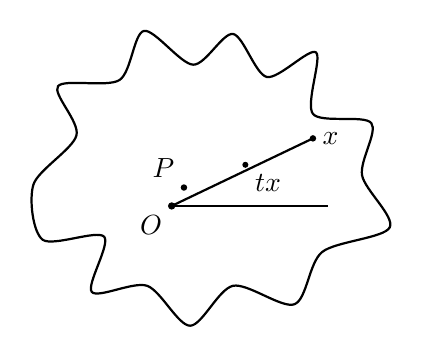
\begin{tikzpicture}[scale=.78]
  \draw[thick] plot[smooth cycle] coordinates {(-2.8,.2) (-2.1,1.0) (-2.4,1.8) (-1.4,1.9) (-1.0,2.7) (-.2,2.15) (.45,2.65) (1.0,1.95) (1.8,2.35) (1.75,1.35) (2.7,1.2) (2.55,.35) (3.0,-.5) (1.9,-.9) (1.45,-1.75) (.45,-1.45) (-.25,-2.1) (-.95,-1.45) (-1.85,-1.55) (-1.65,-.65) (-2.65,-.7)};
  \coordinate (O) at (-.55,-.15);
  \coordinate (P) at (-.35,.15);
  \coordinate (X) at (1.75,.95);
  \coordinate (TX) at (.65,.52);
  \draw[thick] (O)--(X);
  \draw[thick] (O)--(2.0,-.15);
  \fill (O) circle (1.7pt) node[below left] {$O$};
  \fill (P) circle (1.5pt) node[above left] {$P$};
  \fill (X) circle (1.5pt) node[right] {$x$};
  \fill (TX) circle (1.4pt) node[below right] {$tx$};
\end{tikzpicture}
\caption{图7-4-1}
\end{figure}

现在来证(24)式，因为
\[
 d\omega=\frac{\partial a(x)}{\partial x^k}dx^k\wedge dx^{i_1}\wedge\cdots\wedge dx^{i_p}
\]
是一个 $(p+1)$ 形式，相应于 $p$ 变成 $p+1$，(26)应成为
\[
 x^kdx^{i_1}\wedge\cdots\wedge dx^{i_p}
 -\sum_{j=1}^p(-1)^{j-1}x^{i_j}dx^k\wedge dx^{i_1}\wedge\cdots\wedge\widehat{dx^{i_j}}\wedge\cdots\wedge dx^{i_p}.
\]
这是因为 $x^k$ 起了 $x^{i_0}$ 的作用，而原来 $dx^{i_j}$ 是第 $j$ 个因子，现在因为多了一个 $dx^k$ 而成为第 $j+1$ 个因子，所以原来的 $(-1)^{j-1}$ 现在变成了 $(-1)^{(j+1)-1}=-(-1)^{j-1}$。这样
\begin{align*}
 H_{p+1}(d\omega)
 &=H_{p+1}\left(\frac{\partial a}{\partial x^k}dx^k\wedge dx^{i_1}\wedge\cdots\wedge dx^{i_p}\right)\\
 &=\sum_{k=1}^n\left(\int_0^1\frac{\partial a(tx)}{\partial(tx^k)}t^p\,dt\right)
 \left(x^kdx^{i_1}\wedge\cdots\wedge dx^{i_p}-dx^k\wedge\sigma\right).
\end{align*}
上式的 $\sigma$ 仍是(26)式。但是
\begin{align*}
 dH_p(\omega)
 &=d\left[\left(\int_0^1a(tx)t^{p-1}\,dt\right)\sigma\right]\\
 &=d\left(\int_0^1a(tx)t^{p-1}\,dt\right)\wedge\sigma
 +\left(\int_0^1a(tx)t^{p-1}\,dt\right)d\sigma\\
 &=\sum_{k=1}^n\left(\int_0^1\frac{\partial a(tx)}{\partial(tx^k)}t^p\,dt\right)dx^k\wedge\sigma
 +\left(\int_0^1a(tx)t^{p-1}\,dt\right)d\sigma.
\end{align*}
两式相加即有
\[
\begin{aligned}
 H_{p+1}(d\omega)+dH_p(\omega)
 &=\sum_{k=1}^n\left[\int_0^1\frac{\partial a(tx)}{\partial(tx^k)}t^p\,dt\right]x^k
 dx^{i_1}\wedge\cdots\wedge dx^{i_p}\\
 &\quad+\left(\int_0^1a(tx)t^{p-1}\,dt\right)d\sigma.
\end{aligned}
\]
但是
\[
 \sum_{k=1}^n x^k\frac{\partial a(tx)}{\partial(tx^k)}=\frac{\partial}{\partial t}a(tx).
\]
代入上式第一项并用分部积分法知
\begin{align*}
 \text{第一项}
 &=\left.a(tx)t^p\right|_0^1dx^{i_1}\wedge\cdots\wedge dx^{i_p}
 -p\left(\int_0^1a(tx)t^{p-1}\,dt\right)dx^{i_1}\wedge\cdots\wedge dx^{i_p}\\
 &=\omega-p\left(\int_0^1a(tx)t^{p-1}\,dt\right)dx^{i_1}\wedge\cdots\wedge dx^{i_p}.
\end{align*}
第二项中
\[
\begin{aligned}
 d\sigma
 &=\sum_j(-1)^{j-1}dx^{i_j}\wedge dx^{i_1}\wedge\cdots\wedge
 \widehat{dx^{i_j}}\wedge\cdots\wedge dx^{i_p}\\
 &=\sum_j dx^{i_1}\wedge\cdots\wedge dx^{i_p}
 =p\,dx^{i_1}\wedge\cdots\wedge dx^{i_p}.
\end{aligned}
\]
所以
\[
 \text{第二项}=p\left(\int_0^1a(tx)t^{p-1}\,dt\right)dx^{i_1}\wedge\cdots\wedge dx^{i_p}.
\]
两项合并即得定理之证。

庞加莱引理表明，微分流形 $M$ 上的闭形式是否均为恰当形式（从物理上看也就是是否有势存在），取决于 $M$ 的拓扑性质。我们在这里所讲的拓扑性质表现为所谓 de Rham 上同调群 $H^p(M)$。记
\[
 Z^p(M)=\{M\text{ 上的闭的 }p\text{ 形式}\},
\]
并称为 $p$ 维上循环（cocycle）群，这里的“群”是对于 $p$ 形式的加法而言的，因此是阿贝尔（Abel）群（即阿贝群）。又记
\[
 B^p(M)=\{M\text{ 上的恰当 }p\text{ 形式}\},
\]
并称为 $p$ 维上边缘（coboundary）群。其实 $Z^p(M)$ 和 $B^p(M)$ 都不只是群，而且是线性空间，它们的名称中都有一个“上”字，这也不是偶然的。

显然 $B^p(M)\subset Z^p(M)$，其实这就是 $d^2=0$。我们也知道了一般说来 $B^p(M)$ 只是 $Z^p(M)$ 的真子空间——真子群。那么至少要问，$Z^p(M)$ 中确非 $B^p(M)$ 的元“实际”上有多少？准确些说，要考虑商空间或商群 $Z^p(M)/B^p(M)$，并且要问，它的维数是多少？有些什么生成元等等。我们就称这个商空间或商群为 $p$ 阶 de Rham 上同调群，并记作
\[
 H^p(M):=Z^p(M)/B^p(M).
\]
这里 $p\ge0$。$H^p(M)=0$ 就表明 $Z^p(M)=B^p(M)$，亦即每个 $p$ 阶闭形式都是恰当形式。如果 $H^p(M)\ne0$，它既是线性空间，自当有基底。如果 $H^p(M)$ 是有限维的，而基底为 $\omega_1,\ldots,\omega_r$（当然 $\omega_i$ 都是闭形式），这就是说，任一闭形式 $\omega$ 必可写为
\[
 \omega=d\sigma+\sum_{i=1}^r c_i\omega_i,
\]
如果用 $[\omega]$ 表示 $\omega$ 在 $H^p(M)$ 中所属的元，则
\[
 [\omega]=\sum_{i=1}^r c_i[\omega_i].
\]
这样，$M$ 上有“多少”个非恰当的闭形式的问题就得到了解决。$H^p(M)$ 的维数是一个拓扑不变量。实际上，若有微分同胚 $\varphi:M\to N$，则 $H^p(M)\cong H^p(N)$，因此其维数自然不变。这个不变量与 $M$ 的其它不变量例如贝蒂数（Betti numbers）、欧拉示性数（粗略地说就是 $M$ 有多少个“洞”的个数）都有密切关系。de Rham 上同调理论在物理学（例如量子场论）中有重要的应用，这当然超出了本书的范围，下面来举几个例子。

\noindent\textbf{例1}\quad
庞加莱引理告诉我们，若 $M$ 关于某一点是星形的，则 $H^p(M)=0,p>0$。特别是 $\mathbb R^n$ 自然是星形域，所以 $H^p(\mathbb R^n)=0,p>0$。

$p=0$ 又如何？于此，我们有

\noindent\textbf{例2}\quad
若 $M$ 是一个连通流形，可以证明 $H^0(M)\cong\mathbb R$。事实上，因为不存在负阶形式，所以 $B^0(M)=0$ 而 $H^0(M)=Z^0(M)$。我们现在来求 $Z^0(M)$。按定义，$Z^0(M)$ 就是闭的 $0$ 阶形式的空间。但 $M$ 上的 $0$ 阶形式就是 $C^\infty(M)$ 函数，$Z^0(M)=\{f\in C^\infty(M);df=0\}$。因为 $M$ 是连通的，由 $df=0$ 即得 $f=C$ 于 $M$ 上，这里 $C\in\mathbb R$ 是任意实数，这样
\[
 H^0(M)=Z^0(M)=\{C\}\cong\mathbb R.
\]
如果 $M$ 是不连通的，设它有 $r$ 个连通分支，则由 $df=0$ 可知 $f$ 在每个连通分支上取常数值，但在不同分支上可以取不同值，这样 $Z^0(M)$ 之每个元都与一组 $r$ 个实数 $(C_1,\ldots,C_r)$ 对应，故
\[
 H^0(M)=Z^0(M)=\{(C_1,\ldots,C_r)\}\cong\mathbb R^r.
\]

\noindent\textbf{例3}\quad
庞加莱引理讲到，可以收缩为一点的流形上，闭形式均为恰当形式。下面看一个明显不能收缩为一点的流形之例：$S^1$。我们前面一再以
\[
 \omega=\frac{xdy-ydx}{x^2+y^2}
\]
为例。它是闭形式但不是恰当的；找不到一个 $0$ 形式（即 $S^1$ 上的函数 $f$）使 $\omega=df$，就是说，向量场
\[
 \left(-\frac{y}{x^2+y^2},\frac{x}{x^2+y^2}\right)
\]
是没有势函数的——这里讲的是 $S^1$ 上的整体的势函数，而不是 $S^1$ 上任一点的某个邻域中局部的势函数，后者总是存在的，只要这个邻域充分小而且可以收缩为一点即可。现在我们用极坐标来考察这个问题。于是 $S^1$ 成为 $r=1$，$\omega=d\theta$（其实 $d\theta$ 这个记号有毛病，因为 $\theta$ 并非 $S^1$ 上的 $C^\infty$ 函数，但这不会影响以下的讨论，因为可以把 $S^1$ 分成几块坐标邻域来处理）。$H^0(S^1)\cong\mathbb R$ 已如上述，$H^p(S^1)=0$，若 $p>1$，因为 $S^1$ 上没有 $p$ 形式（$p>1$，即 $p=2,3,\ldots$），所以 $H^p(S^1)=0,p>1$。余下只需讨论 $H^1(S^1)$。$S^1$ 是 $1$ 维流形，所以其切空间的基底是 $\{\frac{\partial}{\partial\theta}\}$，而余切空间的基底是 $\{d\theta\}$，而 $S^1$ 上所有的闭 $1$ 形式就是
\[
 \omega=\omega(\theta)d\theta.
\]
这里 $\omega(\theta)$ 是 $\theta$ 的以 $2\pi$ 为周期的 $C^\infty$ 函数。$\omega$ 为恰当形式 $d\sigma$，即存在一个 $\theta$ 的以 $2\pi$ 为周期的 $C^\infty$ 函数 $\sigma$ 使
\[
 \sigma(\theta)=\int_0^\theta\omega(t)dt,
\]
但是上述 $\sigma(\theta)$ 以 $2\pi$ 为周期充分必要条件是
\[
 \int_0^{2\pi}\omega(\theta)d\theta=0.
\]
而一般它是不成立的。为此，我们不考虑 $\omega(\theta)d\theta$ 而考虑 $[\omega(\theta)-c]d\theta$，这里 $c$ 应使
\[
 \int_0^{2\pi}[\omega(\theta)-c]d\theta=0,
\]
即
\[
 c=\frac1{2\pi}\int_0^{2\pi}\omega(\theta)d\theta.
\]
因此 $\omega-cd\theta$ 是恰当形式，即存在 $S^1$ 上的以 $2\pi$ 为周期的 $C^\infty$ 函数 $\sigma(\theta)$ 使
\[
 \omega-cd\theta=d\sigma.
\]
这样我们得到了 $S^1$ 上所有的 $1$ 形式的表达式
\[
 \omega=d\sigma+cd\theta.
\]
（$S^1$ 上所有的 $1$ 形式都是闭的，因为 $S^1$ 是一维的。）于是 $Z^1(S^1)$ 对于 $B^1(S^1)$ 之等价类 $[\omega]=cd\theta$，
\[
 Z^1(S^1)/B^1(S^1)=\{cd\theta\}\cong\mathbb R.
\]
于是得出 $H^1(S^1)\cong\mathbb R$。

这个例子与磁场可以产生感应电流的奥斯特--法拉第的实验有密切的关系，所以我们称 $\omega=\frac{-y\,dx+x\,dy}{x^2+y^2}$ 为奥斯特--法拉第（Oersted--Faraday）形式。我们将在 §6 结束语——麦克斯韦方程组简介中讨论外微分形式与麦克斯韦电磁理论的关系。

\noindent\textbf{6. 重访古典的向量分析}\quad
上节中我们在引入了霍奇 $*$ 算子后把向量代数中的向量和积混合积用外积表示出来，现在我们将继续利用它给向量分析中几个微分运算公式以更简单的证明。

$*$ 算子的引入与空间中对某一度量下的 o.n. 系的选用有密切关系。这个 o.n. 系我们记作 $\{e_1,e_2,\ldots,e_n\}$。因为我们使用了正交坐标系，所以协变与逆变的区别不见了，而我们现在都采用下标。$*$ 算子的公式中经常出现 $p(n-p)+s$，$n$ 是空间维数，在我们的情况下 $n=3$，$p$ 是微分形式的阶数：$0\le p\le n$；当 $n=3$ 时很容易验证，$p(n-p)$ 恒为偶数。如果我们是在欧氏空间中讨论向量，并选用 $(g_{ij})$ 为正定的度量，从而 $s=0$，而有 $(-1)^{p(n-p)+s}=1$。如果我们在闵可夫斯基四维时空中讨论问题，则 $n=4,s=3$，这时 $p(n-p)$ 不一定是偶数，$(-1)^{p(n-p)+s}$ 也不一定是 $1$。

仿照上一节的记号，凡古典的向量分析中的向量均用箭头或黑体字母表示，而现在则用 o.n. 基 $\{e_i\}$ 表示，如
\[
 \mathbf A=A_1\mathbf i+A_2\mathbf j+A_3\mathbf k=A_1e_1+A_2e_2+A_3e_3.
\]
再回忆一下
\begin{equation}
\begin{gathered}
 *\mathbf i=*e_1=e_2\wedge e_3,\qquad *\mathbf j=*e_2=e_3\wedge e_1,\qquad *\mathbf k=*e_3=e_1\wedge e_2,\\
 *(e_2\wedge e_3)=**e_1=e_1,\qquad *(e_3\wedge e_1)=e_2,\qquad *(e_1\wedge e_2)=e_3,\\
 *(e_1\wedge e_2\wedge e_3)=1,\qquad *1=e_1\wedge e_2\wedge e_3.
\end{gathered}
 \tag{27}
\end{equation}
从这里我们还可看到 $**=\operatorname{id}$，所以 $*^{-1}=*$。

现在考虑一个 $0$ 形式 $f$，于是因为 $e_i=dx_i$，
\begin{equation}
 df=\frac{\partial f}{\partial x_1}dx_1+\frac{\partial f}{\partial x_2}dx_2+\frac{\partial f}{\partial x_3}dx_3=\operatorname{grad}f.
 \tag{28}
\end{equation}
对于 $1$ 形式
\[
 \mathbf A=A_1e_1+A_2e_2+A_3e_3=A_1dx_1+A_2dx_2+A_3dx_3,
\]
\[
\begin{aligned}
 d\mathbf A
 &=\left(\frac{\partial A_3}{\partial x_2}-\frac{\partial A_2}{\partial x_3}\right)dx^2\wedge dx^3\\
 &\quad+\left(\frac{\partial A_1}{\partial x_3}-\frac{\partial A_3}{\partial x_1}\right)dx^3\wedge dx^1\\
 &\quad+\left(\frac{\partial A_2}{\partial x_1}-\frac{\partial A_1}{\partial x_2}\right)dx^1\wedge dx^2.
\end{aligned}
\]
所以
\begin{equation}
 *d\mathbf A
 =\left(\frac{\partial A_3}{\partial x_2}-\frac{\partial A_2}{\partial x_3}\right)dx^1
 +\left(\frac{\partial A_1}{\partial x_3}-\frac{\partial A_3}{\partial x_1}\right)dx^2
 +\left(\frac{\partial A_2}{\partial x_1}-\frac{\partial A_1}{\partial x_2}\right)dx^3
 =\operatorname{curl}\mathbf A.
 \tag{29}
\end{equation}
又因
\[
 *\mathbf A=A_1dx^2\wedge dx^3+A_2dx^3\wedge dx^1+A_3dx^1\wedge dx^2,
\]
所以
\begin{equation}
\begin{aligned}
 *d*\mathbf A
 &=*\left[\left(\frac{\partial A_1}{\partial x_1}+\frac{\partial A_2}{\partial x_2}+\frac{\partial A_3}{\partial x_3}\right)
 dx^1\wedge dx^2\wedge dx^3\right]\\
 &=\frac{\partial A_1}{\partial x_1}+\frac{\partial A_2}{\partial x_2}+\frac{\partial A_3}{\partial x_3}
 =\operatorname{div}\mathbf A.
\end{aligned}
 \tag{30}
\end{equation}
于是，梯度、旋度与散度都可以用外微分来表示。由此，外微分的性质将直接给出这些量的相关性质。例如从定理3的性质(i)，即(18)式很容易地导出了以下诸多很容易混淆的公式
\begin{align}
 \operatorname{div}(\operatorname{curl}\mathbf A)&=0, \tag{31}\\
 \operatorname{curl}(\operatorname{grad}f)&=0, \tag{32}\\
 \operatorname{curl}(f\mathbf A)&=f\operatorname{curl}\mathbf A+\operatorname{grad}f\times\mathbf A, \tag{33}\\
 \operatorname{div}(f\mathbf A)&=f\operatorname{div}\mathbf A+\operatorname{grad}f\cdot\mathbf A, \tag{34}\\
 \operatorname{div}(\mathbf A\times\mathbf B)&=\mathbf B\cdot\operatorname{curl}\mathbf A-\mathbf A\cdot\operatorname{curl}\mathbf B. \tag{35}
\end{align}
实际上，\footnote{校勘：底本在公式(34)下方的推导末行将末项误印为“$\operatorname{grad}f\times\mathbf A$”。由公式(34)本身以及 $*(df\wedge *\mathbf A)$ 的类型可知，此处应为内积“$\operatorname{grad}f\cdot\mathbf A$”，今据此改正。}
\[
 *d*(*d\mathbf A)=*d^2\mathbf A=0,
\]
\[
 *d(df)=*d^2f=0,
\]
\[
 *d(f\mathbf A)=f*d\mathbf A+*(df\wedge\mathbf A)=f\operatorname{curl}\mathbf A+\operatorname{grad}f\times\mathbf A,
\]
\[
 *d(*f\mathbf A)=f(*d*\mathbf A)+*(df\wedge *\mathbf A)=f\operatorname{div}\mathbf A+\operatorname{grad}f\cdot\mathbf A,
\]
\[
 *d*(\mathbf A\times\mathbf B)=*d*( *(\mathbf A\wedge\mathbf B))=*d(\mathbf A\wedge\mathbf B)
 =*(d\mathbf A\wedge\mathbf B-\mathbf A\wedge d\mathbf B)
 =\mathbf B\cdot\operatorname{curl}\mathbf A-\mathbf A\cdot\operatorname{curl}\mathbf B.
\]

我们特别注意的当然还是庞加莱引理的应用。为此，假定都是在某一星形区域或一点的邻域中考虑问题。

首先设 $\operatorname{curl}\mathbf A=0$，亦即 $*d\mathbf A=0$ 而有 $d\mathbf A=0$。于是一定位在一个 $0$ 形式即 $C^\infty$ 函数 $f$ 使
\[
 \mathbf A=\operatorname{grad}f.
\]
在物理上，一个向量场 $\mathbf A$ 若适合 $\operatorname{curl}\mathbf A=0$ 的条件，就称为无旋场。于是上面的结论就是无旋场一定有势。但是这只限于区域为星形或为某一点之邻域时成立，否则势将会是多值函数。例3中的奥斯特--法拉第形式（或称奥斯特--法拉第场）就是这样，因为这时有
\[
 \omega=d(\sigma-c\theta),
\]
而 $\theta$ 化到直角坐标系以后成为 $\arctan(y/x)$ 就是一个多值函数。

另外，如果 $\operatorname{div}\mathbf A=0$，亦即 $*d(*\mathbf A)=0$，因此 $*\mathbf A$ 是一个闭 $2$ 形式，这时一定存在一个 $1$ 形式 $\mathbf B$ 使 $*\mathbf A=d\mathbf B$，或 $\mathbf A=*d\mathbf B$。用古典的向量分析语言来表达就是：若 $\operatorname{div}\mathbf A=0$，则必存在一个向量 $\mathbf B$（称为向量势）使 $\mathbf A=\operatorname{curl}\mathbf B$。

讲到向量分析就不能不讲一下拉普拉斯算子，读者们可能都熟悉 $\Delta u=\operatorname{div}\operatorname{grad}u$，而 $\Delta u=0$ 是古典的数学物理中可说是最重要的算子。但是应该指出，它在微分流形上有含意深远的推广。不只是因为它不再是常系数偏微分算子，而且不只是作用在 $0$ 形式（即函数）上，而可以作用在一般的 $p$ 形式上。我们的习惯把它称为 Laplace--Beltrami 算子。它的理论与霍奇的理论和 de Rham 上同调理论密切相关，而且是现代的数学物理的基础之一部分。作用在 $0$ 形式上的拉普拉斯算子以外微分算子 $d$ 为基础，而且要把 $d$ 的“对偶”也同时考虑进来。

我们知道 $d:F^p(M)\to F^{p+1}(M)$，它的“对偶”$\delta$ 则会使微分形式的次数下降一次；$\delta$ 由下面的可交换图式来定义：
\begin{equation}
\begin{gathered}
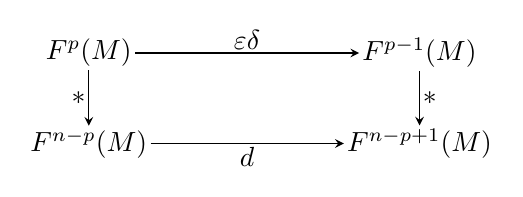
\begin{tikzpicture}[baseline=(current bounding box.center),>=stealth,
  every node/.style={inner sep=1pt}]
  \node (a) at (0,1.15) {$F^p(M)$};
  \node (b) at (4.2,1.15) {$F^{p-1}(M)$};
  \node (c) at (0,0) {$F^{n-p}(M)$};
  \node (d) at (4.2,0) {$F^{n-p+1}(M)$};
  \draw[->] (a)--node[above] {$\varepsilon\delta$} (b);
  \draw[->] (a)--node[left] {$*$} (c);
  \draw[->] (b)--node[right] {$*$} (d);
  \draw[->] (c)--node[below] {$d$} (d);
\end{tikzpicture}\\[-1mm]
\varepsilon=(-1)^p.
\end{gathered}
\tag{36}
\end{equation}
所谓可交换图式即是如果有两条路径起点与终点相同，则沿每一条道路的算子之积（靠近起点的算子先作用），结果相同。因为(36)中有两条路径由左上方的 $F^p(M)$ 通向右上方的 $F^{p-1}(M)$，其一是沿水平方向的 $\varepsilon\delta$，另一条是先用 $*$ 向下通向 $F^{n-p}(M)$，再用 $d$ 向右走到 $F^{n-p+1}(M)$，最后再用霍奇算子的逆 $*^{-1}$ 向上通到 $F^{p-1}(M)$。所以
\[
 \delta=(-1)^p*^{-1}\circ d\circ *,
 \qquad \delta:F^p(M)\to F^{p-1}(M).
\]
以上我们令 $p\ge1$，否则 $F^{p-1}(M)$ 无法定义。除上式外，我们再补充定义 $\delta\omega=0,\omega\in F^0(M)$，于是最后得到，对于 $\omega\in F^p(M)$，
\begin{equation}
 \delta\omega=
 \begin{cases}
 (-1)^p*^{-1}\circ d\circ *\,\omega,&p>0,\\
 0,&p=0.
 \end{cases}
 \tag{37}
\end{equation}
$\delta$ 是 $d$ 的对偶算子。为什么是对偶，我们在讲了积分理论以后就清楚了。

现在我们定义 $\mathbb R^n$ 上的 Laplace--Beltrami 算子为
\begin{equation}
 \Delta\omega=(d\delta+\delta d)\omega,
 \qquad \omega\in F^p(\mathbb R^n),\quad p\ge0.
 \tag{38}
\end{equation}
古典的拉普拉斯算子是 $F^0(\mathbb R^n)$（即 $C^\infty$ 函数）空间上的算子（当然可以推广到甚至是广义函数空间上去）而现在则是由微分形式空间 $F^p(\mathbb R^n)$ 到 $F^p(\mathbb R^n)$ 上的映射。当 $p=0$ 时，注意到这时 $\delta\omega=0$，$\omega\in F^0(\mathbb R^n)$，
\[
 \Delta\omega=\delta d\omega=[-*^{-1}\circ d\circ *\circ d]\omega=-[*\circ d\circ *\circ d]\omega.
\]
这里我们利用了上节(39)式，在 $\mathbb R^n$ 中对于欧几里得度量 $p=0$ 时 $\delta=0$，故 $**=\operatorname{id}$，于是
\[
 \Delta\omega=-\operatorname{div}\operatorname{grad}\omega.
\]
可是现在的 Laplace--Beltrami 算子与古典的拉普拉斯算子相差一个符号，这使它应用起来更方便。因此在现代文献中我们常见到
\[
 \Delta=-\left[\left(\frac{\partial}{\partial x^1}\right)^2+\cdots+\left(\frac{\partial}{\partial x^n}\right)^2\right].
\]
我们还要问，对 $p>0$ 的 $F^p(\mathbb R^3)$，$\Delta\omega$ 是什么？一个常用的情况是 $\omega\in F^1(\mathbb R^3)$，我们就记为 $\omega=\mathbf u$。这时，因 $d\omega\in F^2(\mathbb R^3)$，故
\[
 \delta d\omega=*d*d\omega=\operatorname{curl}\operatorname{curl}\mathbf u,
\]
而
\[
 d\delta\omega=-d*d*\omega=-\operatorname{grad}\operatorname{div}\mathbf u.
\]
另一方面我们可以直接计算 $\Delta\omega$ 如下：不妨设 $\omega=u_i dx^i$，于是经过不太复杂的计算有
\[
 \Delta\omega=-\left[\left(\frac{\partial}{\partial x^1}\right)^2+\left(\frac{\partial}{\partial x^2}\right)^2+\left(\frac{\partial}{\partial x^3}\right)^2\right]\mathbf u,
\]
即对 $\mathbf u$ 之每个分量作古典的拉普拉斯算子并反号。于是有
\begin{equation}
 \operatorname{curl}\operatorname{curl}\mathbf u
 =\operatorname{grad}\operatorname{div}\mathbf u-\nabla^2\mathbf u.
 \tag{39}
\end{equation}
这里我们采用了古典的微积分教本中常用的记法：$\nabla^2=\nabla\cdot\nabla$，而 $\nabla=\frac{\partial}{\partial x^1}\mathbf i+\frac{\partial}{\partial x^2}\mathbf j+\frac{\partial}{\partial x^3}\mathbf k$，这样记就不会对 $\Delta$ 的符号产生误会了。(39)式如果按古典的讲法来证明，并不是一件容易事。

上面我们利用外微分形式特别是霍奇 $*$ 算子，非常清楚地讲了古典的“场论”在 $\mathbb R^n$ 中的许多公式。但是如果换其它坐标系，更容易看出它的好处来。上一节已经看得很明白，在任一度量 $(g_{ij})$ 下，只要找到了 o.n. 系 $\{e^1,\ldots,e^n\}$ 就可以定义 $*$ 算子，因此也就可能定义 $\operatorname{grad},\operatorname{curl}$ 与 $\operatorname{div}$ 等等。在 o.n. 基底下，度量矩阵 $(g_{ij})$ 一定是对角矩阵，这是因为
\[
 g_{ij}=\langle e_i,e_j\rangle,
\]
所以 $i\ne j$ 时 $g_{ij}=0$。这样
\begin{equation}
 ds^2=H_1(dx^1)^2+\cdots+H_n(dx^n)^2.
 \tag{40}
\end{equation}
如果取度量为正定的，则有 $H_i>0$，而且 $H_1\cdots H_n=g=\det(g_{ij})>0$。所以只要令
\[
 e^i=\sqrt{H_i}\,dx^i,
 \qquad e_i=\frac1{\sqrt{H_i}}\frac{\partial}{\partial x^i},
\]
就可以得到所需的 o.n. 系，面对它们定义 $*$ 算子。下面我们限于三维的具有正定度量的流形 $M$，即三维黎曼流形，并以 $(x^1,x^2,x^3)$ 为其局部坐标。所以有时我们也把 $M$ 直接写成 $\mathbb R^3$。

于是对于 $\omega\in F^0(M)$（我们习惯用 $f$ 表示一个 $0$ 微分形式，因为它确实就是一个函数），
\[
 df=\frac{\partial f}{\partial x^i}dx^i
 =\frac1{\sqrt{H_i}}\frac{\partial f}{\partial x^i}e^i,
\]
因此我们应定义
\begin{equation}
 \operatorname{grad}f=
 \left(\frac1{\sqrt{H_1}}\frac{\partial f}{\partial x^1},\ldots,
 \frac1{\sqrt{H_n}}\frac{\partial f}{\partial x^n}\right).
 \tag{41}
\end{equation}
往下，如果 $\omega\in F^1(M)$，$\omega=A_ie^i$ 或者写为 $\omega=\mathbf A$，我们有
\[
 \omega=(A_i\sqrt{H_i})dx^i.
\]
在现在的情况有
\begin{align*}
 d\omega
 &=\left(\frac{\partial(A_3\sqrt{H_3})}{\partial x^2}-\frac{\partial(A_2\sqrt{H_2})}{\partial x^3}\right)dx^2\wedge dx^3\\
 &\quad+\left(\frac{\partial(A_1\sqrt{H_1})}{\partial x^3}-\frac{\partial(A_3\sqrt{H_3})}{\partial x^1}\right)dx^3\wedge dx^1\\
 &\quad+\left(\frac{\partial(A_2\sqrt{H_2})}{\partial x^1}-\frac{\partial(A_1\sqrt{H_1})}{\partial x^2}\right)dx^1\wedge dx^2.
\end{align*}
而
\begin{equation}
 *d\omega=
 \frac1{\sqrt{H_2H_3}}
 \left(\frac{\partial(A_3\sqrt{H_3})}{\partial x^2}-\frac{\partial(A_2\sqrt{H_2})}{\partial x^3}\right)e^1+\cdots.
 \tag{42}
\end{equation}
因此，我们应该有
\begin{equation}
 \operatorname{curl}\mathbf A=
 \frac1{\sqrt{H_2H_3}}
 \left(\frac{\partial(A_3\sqrt{H_3})}{\partial x^2}-\frac{\partial(A_2\sqrt{H_2})}{\partial x^3}\right)e^1+\cdots.
 \tag{43}
\end{equation}
下面没有写出的项均可由第一项用轮换对称得出。最后看 $\operatorname{div}\mathbf A=*d*\mathbf A$，因为
\[
 *\mathbf A=A_1e^2\wedge e^3+A_2e^3\wedge e^1+A_3e^1\wedge e^2
\]
\[
 =A_1\sqrt{H_2H_3}\,dx^2\wedge dx^3+A_2\sqrt{H_3H_1}\,dx^3\wedge dx^1
 +A_3\sqrt{H_1H_2}\,dx^1\wedge dx^2,
\]
\[
 d*\mathbf A=
 \left(\frac{\partial}{\partial x^1}A_1\sqrt{H_2H_3}
 +\frac{\partial}{\partial x^2}A_2\sqrt{H_3H_1}
 +\frac{\partial}{\partial x^3}A_3\sqrt{H_1H_2}\right)dx^1\wedge dx^2\wedge dx^3
\]
\[
 =\frac1{\sqrt{H_1H_2H_3}}
 \left(\frac{\partial}{\partial x^1}A_1\sqrt{H_2H_3}+\cdots\right)e^1\wedge e^2\wedge e^3.
\]
所以
\begin{equation}
 \operatorname{div}\mathbf A=
 \frac1{\sqrt{H_1H_2H_3}}
 \left(\frac{\partial}{\partial x^1}A_1\sqrt{H_2H_3}+\cdots\right).
 \tag{44}
\end{equation}

最后我们来看 Laplace--Beltrami 算子，对于 $f\in F^0(M)$，有
\begin{align}
 \Delta f&=(d\delta+\delta d)f=\delta df=-*d*df=-\operatorname{div}\operatorname{grad}f\notag\\
 &=-\frac1{\sqrt{H_1H_2H_3}}
 \left\{\frac{\partial}{\partial x^1}\left(\sqrt{\frac{H_2H_3}{H_1}}\frac{\partial f}{\partial x^1}\right)+\cdots\right\}.
 \tag{45}
\end{align}
这些公式有一个常见的用处，即在 $\mathbb R^3$ 中引入球坐标
\[
 x^1=r\sin\theta\cos\varphi,\qquad
 x^2=r\sin\theta\sin\varphi,\qquad
 x^3=r\cos\theta
\]
时，很容易算出
\[
 ds^2=dr^2+r^2d\theta^2+r^2\sin^2\theta\,d\varphi^2.
\]
不妨以 $(r,\theta,\varphi)$ 为 $(x^1,x^2,x^3)$，现在我们知道不应该令
\[
 \operatorname{grad}f=\left(\frac{\partial f}{\partial r},\frac{\partial f}{\partial\theta},\frac{\partial f}{\partial\varphi}\right),
\]
因为这个“记号”没有上面这些公式表示的几何性质，而应该注意现在应可得
\[
 H_1=1,\qquad H_2=r^2,\qquad H_3=r^2\sin^2\theta,
\]
而有
\begin{equation}
 \operatorname{grad}f=
 \left(\frac{\partial f}{\partial r},\frac1r\frac{\partial f}{\partial\theta},\frac1{r\sin\theta}\frac{\partial f}{\partial\varphi}\right).
 \tag{46}
\end{equation}
对于一个向量 $\mathbf A$，在坐标 $(r,\theta,\varphi)$ 中应该先把它写成
\[
 \mathbf A=A_1dr+A_2(r\,d\theta)+A_3(r\sin\theta)d\varphi,
\]
然后用(43)和(44)可得
\begin{equation}
\begin{aligned}
 \operatorname{curl}\mathbf A
 &=\frac1{r^2\sin\theta}
 \left(\frac{\partial[A_3(r\sin\theta)]}{\partial\theta}-\frac{\partial(A_2r)}{\partial\varphi}\right)dr\\
 &\quad+\frac1{r\sin\theta}
 \left(\frac{\partial A_1}{\partial\varphi}-\frac{\partial[A_3(r\sin\theta)]}{\partial r}\right)d\theta\\
 &\quad+\frac1r
 \left(\frac{\partial(A_2r)}{\partial r}-\frac{\partial A_1}{\partial\theta}\right)d\varphi,
\end{aligned}
 \tag{47}
\end{equation}
\begin{equation}
 \operatorname{div}\mathbf A=
 \frac1{r^2\sin\theta}
 \left\{\frac{\partial}{\partial r}(A_1r^2\sin\theta)
 +\frac{\partial}{\partial\theta}(A_2r\sin\theta)
 +\frac{\partial}{\partial\varphi}(A_3r)\right\}.
 \tag{48}
\end{equation}
而拉普拉斯算子（注意符号）是
\begin{equation}
\begin{aligned}
 \Delta f
 &=-\left[\frac1{r^2\sin\theta}\frac{\partial}{\partial r}
 \left(r^2\sin\theta\frac{\partial f}{\partial r}\right)
 +\frac{\partial}{\partial\theta}\left(\sin\theta\frac{\partial f}{\partial\theta}\right)
 +\frac{\partial}{\partial\varphi}\left(\frac1{\sin\theta}\frac{\partial f}{\partial\varphi}\right)\right]\\
 &=-\left[\frac1{r^2}\frac{\partial}{\partial r}\left(r^2\frac{\partial f}{\partial r}\right)
 +\frac1{\sin\theta}\frac{\partial}{\partial\theta}\left(\sin\theta\frac{\partial f}{\partial\theta}\right)
 +\frac1{\sin^2\theta}\frac{\partial^2f}{\partial\varphi^2}\right].
\end{aligned}
 \tag{49}
\end{equation}
